% Schnelles Übersetzen scheitert wegen µm in Titel Bach.2012!!
\documentclass[12pt,a4paper,onecolumn,draft]{scrartcl}
\usepackage[utf8]{inputenc}
\usepackage{adjustbox}
\usepackage{amsfonts}
\usepackage{amsmath}
\usepackage{amssymb}
\usepackage{array}
\usepackage[ngerman]{babel}
\usepackage[backend=biber,natbib=true,hyperref=true,
			style=draft,maxnames=2,maxbibnames=2, isbn=false]{biblatex} % STYLE draft SPÄTER NOCH GEGEN authoryear TAUSCHEN!!!!!!
\usepackage{caption, booktabs}
\usepackage{chngcntr} % Damit Zählungen von Abb und Co innerhalb sections mögl
\usepackage{csquotes}
\usepackage{float}
\usepackage[left=2.5cm,right=2.5cm,top=2.5cm,bottom=2.5cm,head=14.5pt]{geometry}
\usepackage[toc,acronym,nonumberlist,translate=babel]{glossaries}
\usepackage{graphicx}
\usepackage{grffile} % to allow underscores in filenames (pics&co)
\usepackage{hyperref}
\usepackage{lmodern}
\usepackage{makecell}
\usepackage{mathtools}
\usepackage{paralist}
\usepackage{pdfpages}
\usepackage[section]{placeins} % to keep figures in section
\usepackage{scrlayer-scrpage} % Zur Anpassung der Kopf- und Fußzeilen
\usepackage{subfig}
\usepackage{tabularx}
%\usepackage[scaled]{uarial} % Schriftart
\usepackage{underscore}
\usepackage{url}
\usepackage{wrapfig}

\addbibresource{literatur.bib} %% Einbinden der bib-Datei
\DefineBibliographyStrings{ngerman}{
	andothers = {{et\,al\adddot}},}

\def\theequation{\thesection.\arabic{equation}} % Formeln beginnen mit Abschnittssnummer
\linespread{1.0} % Zeilenabstand
\pagestyle{scrheadings}
\clearpairofpagestyles % Löschen der Platzhalter
\counterwithin{figure}{section} % damit figure je section neu gezählt werden

\newcommand*\mytitle{Auswirkungen eines extremen Staubereignisses auf die Produktion von Phytoplankton im südlichen Ozean}
\newcommand*\mysubtitle{Bachelorarbeit}
\newcommand*\myauthor{Marco Schulz}
\newcommand*\mydate{05.05.2021}
\newcommand{\cotwo}{CO\textsubscript{2}}

\begin{document}
\begin{titlepage}
\begin{center}
{\LARGE \textsc{\mysubtitle}} \bigskip \\
{\huge \textsf{\mytitle}} \bigskip \\
{\Large \myauthor \ - Matrikelnummer 7345692} \smallskip \\
{\Large Fassung vom \mydate} \bigskip \\
\begin{figure}[H]
\centering

\includegraphics[width=60mm]{bilder/unilogo.png}
\end{figure}
\bigskip
{\Large Institut für Geophysik und Meteorologie}
\bigskip
{\Large \\ Universität zu Köln}
\vspace{4cm}
\\
\end{center}
\begin{tabbing}
Erstgutachter: \quad  \= Prof. Yaping Shao (yshao@meteo.uni-koeln.de) \\[2ex]
Zweitgutachter:  \>  Dr. Hendrik Elbern (he@eurad.uni-koeln.de)
\end{tabbing}
\end{titlepage}
\setcounter{page}{2}
\ofoot{\pagemark}
\chead{{\small \mytitle}}
\automark{section}
\tableofcontents
\newpage
\begin{abstract}
Klima verändert sich. Aktuell Eiszeitalter. Glaziale, Interglaziale abwechselnd. Bekannt (aus Eisbohrkernen), dass geringe \cotwo -Konzentration in Atmosphäre während Glazialen. Deckt sich mit den geringen Temperaturen. Wohin das ganze \cotwo ? Phytoplankton sorgt für $50\%$ des jährlichen \cotwo -Austauschs \citep{Field.1998} und erzeugen etwa 50 gt organischen Kohlenstoff pro Jahr \citep{Emerson.2009}. Phytoplankton benötigt \cotwo \ zum Wachsen, wodurch dieses zu Biomasse konvertiert wird. Somit bei erhöhten Phytoplankton weniger \cotwo . Warum wächst Phytoplankton dann nicht beständig, bis alles \cotwo\ aufgebraucht? Weitere limitierende Faktoren, da zur Fotosynthese weitere Nährstoffe benötigt werden. Nitrat und Phosphate als Nährstoffe, auch von Tiefsee. \citet{Martin.1988} zeigen, dass Eisen limitierender Faktor. Eiseneintrag hauptsächlich aus Staub. Wenige Staubquellen in Südhemisphäre bzw. südl. Ozean (vgl. China/Sahara). Dadurch Eisenmangel, hingegen reich an Nitraten und Phosphaten aufgrund Upwelling (aufgrund Ekmantransport der zyklonalen Zirkumpolarströmung). Falls dann doch größere Eisendeposition, Phytoplankton-Blüten. Dies als mögliche Erklärung für geringe \cotwo - Konzentrationen während Glazialen (Modelle zeigen, dass dies ungefähr die Hälfte des \cotwo \ Rückgangs erklären könnte. Etwa 16 gt Kohlenstoff werden aktuell pro Jahr durch die biologische Pumpe im Ozean archiviert \citep{Falkowski.1998}. Wenn diese Hypothese angenommen, dann bei größeren Staub-Events (kleine Zeitskala) vermehrtes Phytoplankton Wachstum wahrscheinlich. Ein großes Event 2009 in Australien. Dieses soll in dieser Arbeit genauer untersucht werden. Abgleich Staub- bzw. Eisendeposition mit Entwicklung Phytoplankton (bzw. Chlorophyll-$\alpha$). Dazu benutze Kölner WRF-Staub-Weiterentwicklung. Vergleich mit Satellitenbildern. Nutze verschiedene Verfahren der Statistik. Berücksichtige Ozeanzirkulation und Wind. Falls Zusammenhang gezeigt werden kann dann Hypothese wahrscheinlich. Wäre weiteres Indiz für Eisenhypothese. Wurde schonmal gemacht \citep{Gabric.2016}. Prüfung des Kölner Modells. Zusammenhang $\Rightarrow$ ggf. ebenfalls Hinweis dass Modell gut.
\end{abstract}
\section{Einleitung}
Das in allen Weltmeeren präsente Phytoplankton ist für ungefähr die Hälfte des Sauerstoff- und Kohlenstoffdioxidaustauschs verantwortlich \citep{Emerson.2009} und präsentiert damit möglicherweise die wichtigste Spezies unseres Planeten. Zu verstehen, wann, wo und in welcher Größenordnung Kohlenstoffdioxid (\cotwo) von der Atmosphäre aufgenommen oder abgegeben wird, ist gleichzeitig auch heute noch eine der großen Herausforderungen der Klimaforschung. Das Modell vom sogenannten Kohlenstoffkreislauf wird laufend weiterentwickelt und detaillierter. Im Rahmen dieser Arbeit wird ein besonders starker Staubsturm und dessen mögliche temporäre Auswirkung auf diesen Kreislauf durch eine gesteigerte Produktion von Phytoplankton untersucht. Das Staubereignis wird mithilfe eines speziell hierfür angepassten \textit{Weather Research and Forecasting Model} (WRF) simuliert. Falls ein entsprechender Einfluss abgeleitet werden kann, würde dies implizit die 1990 von John H. Martin aufgestellte Eisenhypothese weiter unterstützen, welche unser Verständnis der Klimaprozesse auf geologischen Zeitskalen entscheidend verbessert hat. Der gegenteilige Fall wäre ein Indiz dafür, dass die Hypothese an weitere Bedingungen geknüpft ist oder gar andere Prozesse dominieren.  \\

Im ersten Schritt wird hierzu in Kapitel \ref{sec:Theorie} der aktuelle Stand des Wissens dargestellt und erläutert, in welchem Zusammenhang Staub, Phytoplankton und letztlich die Speicherung des Kohlenstoffs stehen und welche besonderen Effekte bei der Interpretation unbedingt zu berücksichtigen sind.  Im ersten Teil dieses theoretischen Fundaments (Kapitel  \ref{sec:Klima}) soll insbesondere motiviert werden, warum es nicht zuletzt angesichts der aktuellen anthropogenen Verstärkung der Klimaerwärmung so wichtig ist, die Auswirkungen von Kohlenstoffdioxidkonzentrationen in der Atmosphäre und deren Treiber genau zu verstehen. Anschließend wird in Kapitel \ref{sec:Eisenhypothese} die wegweisende Eisenhypothese \citep{Martin.1990} vorgestellt und die damit verbundene besondere Rolle des südlichen Ozeans erläutert. Um die Implikationen dieser Hypothese prüfen zu können, ist ein genaues Verständnis von der Entwicklung des Phytoplanktons und deren zahlreiche Folgen und Komplikationen erforderlich, insbesondere der Limitierung durch Eisen  (Kapitel \ref{sec:Phytoplankton}). Träger für ebendieses Element ist Staub. Folglich wird im darauffolgenden Kapitel \ref{sec:Staub} speziell für den Kontinent Australien der eng mit dem Kohlenstoffkreislauf verbundene Staubkreislauf mit typischen Eigenschaften, Staubquellen und Zirkulationsmustern  präsentiert. Zum Abschluss des Kapitels wird schließlich noch der einzigartige Staubsturm analysiert, dessen Auswirkungen auf die Produktion von Phytoplankton im Rahmen dieser Arbeit untersucht werden sollen. Dieses von den Medien als \textit{Red Dawn} betitelte Ereignis nahm in Sydney am 23. September 2009 seinen Höhepunkt. \\

In Kapitel \ref{sec:Methoden} wird anschließend vorgestellt, mithilfe welcher Methoden und Daten der Staubsturm und dessen Auswirkungen genauer untersucht werden können. Das Programm bzw. Wettermodell WRF wurde um ein Modul für Emission, Transport und Ablagerung von Staub erweitert und ermöglicht so eine zeitlich und räumlich höhere Auflösung des Staubsturms als die vorhanden Beobachtungsdaten. Der damit modellierte Staubeintrag in den benachbarten Ozean kann die chemische Zusammensetzung des Meerwassers entsprechend verändern und die Produktion von Phytoplankton fördern. Zur Bewertung dieser potentiellen Veränderungen wird die zeitliche Veränderung der Phytoplanktonkonzentrationen aus satellitengestützten Messungen des natürlichen Farbstoffs \textit{Chlorophyll a} abgeleitet. Zur Prüfung eines Zusammenhangs zwischen Staub und Phytoplanktonkonzentrationen werden verschiedene statistische Methoden in Erwägung gezogen.\\

Abschließend werden die Ergebnisse präsentiert und bei Berücksichtigung vergleichbarer Analysen aus der Literatur interpretiert. Insbesondere werden dabei die Ergebnisse von \citet{Gabric.2016} herangezogen. In dieser Arbeit wurden  für annähernd den gleichen Zeitraum mit anderen Methoden die Auswirkungen aus das tasmanische Meer untersucht.  \citet{Gabric.2016} schließen mit dem Fazit, dass sich die Phytoplanktonkonzentrationen in bestimmten Regionen des tasmanischen Meeres in Folge des Staubereignisse signifikant erhöhen und legen in der Begründung einen besonderen Fokus auf den Effekt der  \textit{feuchten} Ablagerung von Staubpartikeln. Mögliche Vorteile und Gründe für abweichende Ergebnisse der vorliegenden Arbeit sind das weiterentwickelte Staubmodell, verbesserte tägliche Chlorophyll-a Daten, klarere statistische Methoden und die Erweiterung des Untersuchungsgebiets auf den südlichen Ozean.

\section{Theoretischer Kontext} \label{sec:Theorie}
Staub nimmt auf verschiedene Weisen Einfluss auf das Klima. Der möglicherweise direkteste Einfluss wirkt auf die Energiebilanz. Staub ist mobil und kann vielfältige Strukturen und Formen annehmen. Durch die Ablagerung auf Oberflächen werden deren Albedo und Absorptionseigenschaften verändert. Während des Transports in der Atmosphäre kann Staub Strahlung auf noch komplexere Weise absorbieren, reflektieren, brechen, streuen oder emittieren \citep{Shao.2011} und somit Temperaturverteilung und -gradienten beeinflussen. Einen deutlich indirekteren und verzögerten, aber nicht minder wichtigen Einfluss nimmt Staub auf den Kohlenstoffkreislauf, welcher wiederum wichtige Auswirkungen auf das Klima hat. In diesem Abschnitt soll einer dieser Treiber mit den entsprechenden Zwischenschritten in umgekehrter Reihenfolge der Wirkungskette (Staubsturm$\rightarrow$Eisen$\rightarrow$Phytoplankton$\rightarrow$\cotwo $\rightarrow$Klima) erläutert werden. Jedes Unterkapitel erläutert die jeweilige Verbindung zum vorangegangenen Kapitel und beinhaltet wichtige Aspekte, die bei der späteren Interpretation des Zusammenhangs zwischen Staubsturm und Phytoplanktonproduktion berücksichtigt werden müssen. Im ersten Kapitel \ref{sec:Klima} wird an den dafür grundlegenden Zusammenhang zwischen dem Treibhausgas \cotwo \ und den erdgeschichtlichen sowie aktuellen Temperaturentwicklungen erinnert. Daraufhin beschreibt \ref{sec:Eisenhypothese} die für diese Arbeit fundamentale Eisenhypothese mit der besonderen Rolle des südlichen Ozeans. Zentrales Objekt dieser Hypothese ist das Phytoplankton und dessen mögliche Limitierung durch das Element Eisen sowie die Fähigkeit der sogenannten \textit{Biologischen Pumpe} Kohlenstoff dauerhaft aus dem Kreislauf zu entfernen (\ref{sec:Phytoplankton}). Zum Abschluss wird das eigentliche Staubereignis in einem für den australischen Kontinent allgemeinen Kontext beschrieben. Zusammen bieten die Kapitel eine grundsätzliche Übersicht des aktuellen Stands der Wissenschaft zur potentiellen Wirkung eines Staubereignisses auf den Kohlenstoffkreislauf.
\subsection{Kohlenstoffdioxid und die Klimageschichte} \label{sec:Klima}
Dass Treibhausgase wie \cotwo \ einen Einfluss auf die Temperaturverteilung in der Atmosphäre haben, ist allgemein bekannt und bereits seit langer Zeit mithilfe verschiedenster Beobachtungen, Modelle und theoretischen Konzepten wissenschaftlich hinreichend belegt. Dies und der aktuelle Einfluss des Menschen durch die Erhöhung der \cotwo \ Konzentrationen durch Emission fossiler Brennstoffe wurde schon 1990 im ersten Assessment Report des \textit{Intergovernmental Panel on Climate Change} (IPCC) auf Basis einer Zusammenstellung der damals aktuellen Kenntnisse kondensiert, dokumentiert und entsprechend politischen Entscheidungsträgern verfügbar gemacht. Aufgrund der massiven potentiellen Auswirkungen von abrupten Klimaveränderungen \citep{IPCCpol.2018} ist es von besonderer Bedeutung, die Prozesse genau zu verstehen und bestmöglich zu quantifizieren. Da das Klima auf geologischen Zeitskalen von jeher eine Veränderung durchläuft und die entsprechenden treibenden Prozesse teilweise auch heute noch präsent sind, ist der Blick in die Vergangenheit dabei von unschätzbarem Wert. Derartige Rückblicke sind insbesondere mithilfe von Eisbohrkernen möglich, in welchen mit zunehmender Tiefe die Atmosphären der jeweiligen weiter zurückliegenden Zeiten archiviert wurden. Dies erlaubt direkte Rückschlüsse auf die Konzentrationen von Gasen als auch indirekte Berechnungen von bspw. der Temperaturentwicklung. In Abbildung \ref{fig:icecore} sind entsprechend aus einem Bohrkern aus der Antarktis Zeitreihen für die (nach Wasser) beiden ausschlaggebendsten Treibhausgase \cotwo \ und Methan (CH$_4$) zusammen mit der Temperaturanomalie und den Staubkonzentrationen dargestellt. Bereits ohne weitere statistische Analysen ist auffällig, dass die drei ersten Größen \cotwo , CH$_4$ und Temperatur miteinander korrelieren. In regelmäßigen Abständen von etwa 100.000 Jahren erreichen alle drei Zeitreihen praktisch gleichzeitig vergleichsweise kurze lokale Maxima, auf welche etwas längere Phasen mit geringen Konzentrationen/Temperaturen folgen. Diese Periode repräsentiert genau einen Zyklus des aktuellen Eiszeitalters, in welchem sich Warmzeiten (Interglaziale) und Kaltzeiten (Glaziale bzw. ugs. Eiszeiten) abwechseln. Aktuell befinden wir uns in einer Warmzeit mit hohen Treibhausgaskonzentrationen. Entgegen der Abbildung liegen die derzeitigen (März 2021) \cotwo \ Konzentrationen aufgrund der anthropogenen Emissionen bei etwa 416 parts per million (ppm) \citep{NASA.06.05.2021}; das dortige Jahr 0 liegt mehrere Jahrzehnte in der Vergangenheit \citep{Luthi.2008}. Der statistische Zusammenhang zwischen Kohlenstoffdioxidkonzentrationen und der mittleren Temperatur an der Erdoberfläche ist also klar.  Trotz dieser Indizien ist es allerdings weiterhin schwierig, aus den verfügbaren Zeitreihen rein statistisch eine klare Kausalität zu beweisen. Dies impliziert, dass die beobachtete Korrelation theoretisch auch aufgrund eines anderen externen Treibers verursacht sein könnte, der beide Größen \cotwo -Konzentration und mittlere Temperaturen beeinflusst. Allerdings geben neuere statistische Methoden \citep{Stips.2016} weitere Indizien für die durch Beobachtungen und Experimente ohnehin bestätigte Annahme , dass beide Variablen kausal zusammenhängen. Für die jüngere Vergangenheit seit Beginn des Industriezeitalters gilt als praktisch sicher, dass die anthropogenen Emissionen von Treibhausgasen zu der gemessenen Erhöhung der globalen Durchschnittstemperatur geführt haben.  \\

Weitere Analysen von \citet{Stips.2016} geben Hinweise darauf, dass der kausale Zusammenhang über größere Zeiträume in der Vergangenheit umgekehrt gewesen sein könnte, dass also steigende oder sinkende Temperaturen zu einer Zu- bzw. Abnahme der \cotwo Konzentrationen geführt haben. Dies impliziert einen wechselseitigen Zusammenhang, wobei der Einfluss von Temperaturen auf Treibhausgaskonzentrationen wesentlich träger, also auf geologischen Zeitskalen funktioniert, andersherum aber \textit{kurzfristige} Reaktionen möglich sind.  Auf sehr großen Zeitskalen (10-100 Millionen Jahre) soll insbesondere die Plattentektonik und die damit verbundenen veränderten Verwitterungsprozesse zu Veränderungen in der \cotwo \ -Bilanz geführt haben. Die jüngeren und regelmäßigen Veränderungen von \cotwo \ und Temperatur auf Zeitskalen von eher 10 bis 100.000 Jahren, welche aus den Untersuchungen der Eisbohrkerne abgleitet werden konnten, werden hingegen auf kurzfristigere Prozesse aufgrund von Modifikationen in der Ozeanzirkulation und biologischen Prozessen (an Land und in Meer) zurückgeführt \citep{Emerson.2009}. Hierzu gibt auch die vierte Variable der abgeleiteten Staubkonzentrationen in Abbildung \ref{fig:icecore} weitere Hinweise. Diese Zeitreihe der Staubkonzentrationen hat genau dort Maxima, wo die übrigen Variablen geringe Werte aufweisen. Dies impliziert, dass Emission, Transport und Ablagerung von Staub möglicherweise ebenfalls von Klimaveränderungen beeinflusst werden. Analysen der Zeitreihen zeigen genauer, dass der Staubfluss und die Temperatur während der Glaziale korrelieren, was während der Interglaziale nicht beschrieben werden kann \citep{Lambert.2008}. Eine mögliche Erklärung für diesen Zusammenhang des beispielhaften Bohrkerns aus der Ostantarktis ist, dass die südamerikanischen Staubquellen während der Kaltphasen verstärkt wurden und gleichzeitig die Aufenthaltszeit der Staubpartikel in der Atmosphäre aufgrund des schwächeren Wasserkreislaufs zugenommen hat, was letztlich zu stärkeren Ablagerungen während dieser Zeiten führte \citep{Lambert.2008}. Entscheidend ist, dass zwischen Staub und Klima offenbar ein Zusammenhang besteht. Ein solcher Zusammenhang führte schließlich zu John Martin's Formulierung der Eisenhypothese. Allgemein wird angenommen, dass
die (inter)glazialen \cotwo -Schwankungen durch eine Kombination aus \textit{Eisendüngung}, Veränderungen bei den Karbonatkompensationen (Auflösung von Calcit und Aragonit mit  \cotwo \ zu Calcium und Bikarbonat in der Tiefsee) und Ventilation des südlichen Ozeans \citep{Lambert.2012} gesteuert werden. Die Analyse der Phasenverschiebung zwischen Staubflüssen und \cotwo -Konzentrationen von \citet{Lambert.2012} zeigen allerdings, dass die Eisendüngung des südlichen Ozeans durch Staub jedenfalls gegen \textit{Ende} der letzten 9 Glaziale offenbar nicht der dominante Faktor für den Anstieg der \cotwo -Konzentrationen war. Der Staubfluss erreicht stets etwa 4.000 Jahre früher die für Interglaziale typischerweise  geringen Werte während sich \cotwo \ und Temperatur noch verändern (ansteigen) können. Offen bleibt, wie hoch der Beitrag tatsächlich ist und ob ggf. umgekehrt die Eisendüngung zu \textit{Beginn} der Glaziale dennoch ein dominanter Faktor zur \textit{Reduzierung} der Konzentrationen sein kann. \citet{MartinezGarcia.2009} folgern hierzu anhand der zeitlichen Eintretens der Effekte allerdings ebenfalls , dass der ursächliche Anstoß des starken Abfalls der \cotwo -Konzentrationen eher durch physikalische Prozesse erfolgte, wie Veränderungen der antarktischen Meereisausdehnung, Stratifizierung des Oberflächenwassers und die geographische Ausdehnung der sogenannten \textit{Westerlies}. Dennoch wird der Eisendüngung weiterhin ein maßgeblicher Anteil zugeschrieben.

\begin{figure}[ht]
\centering
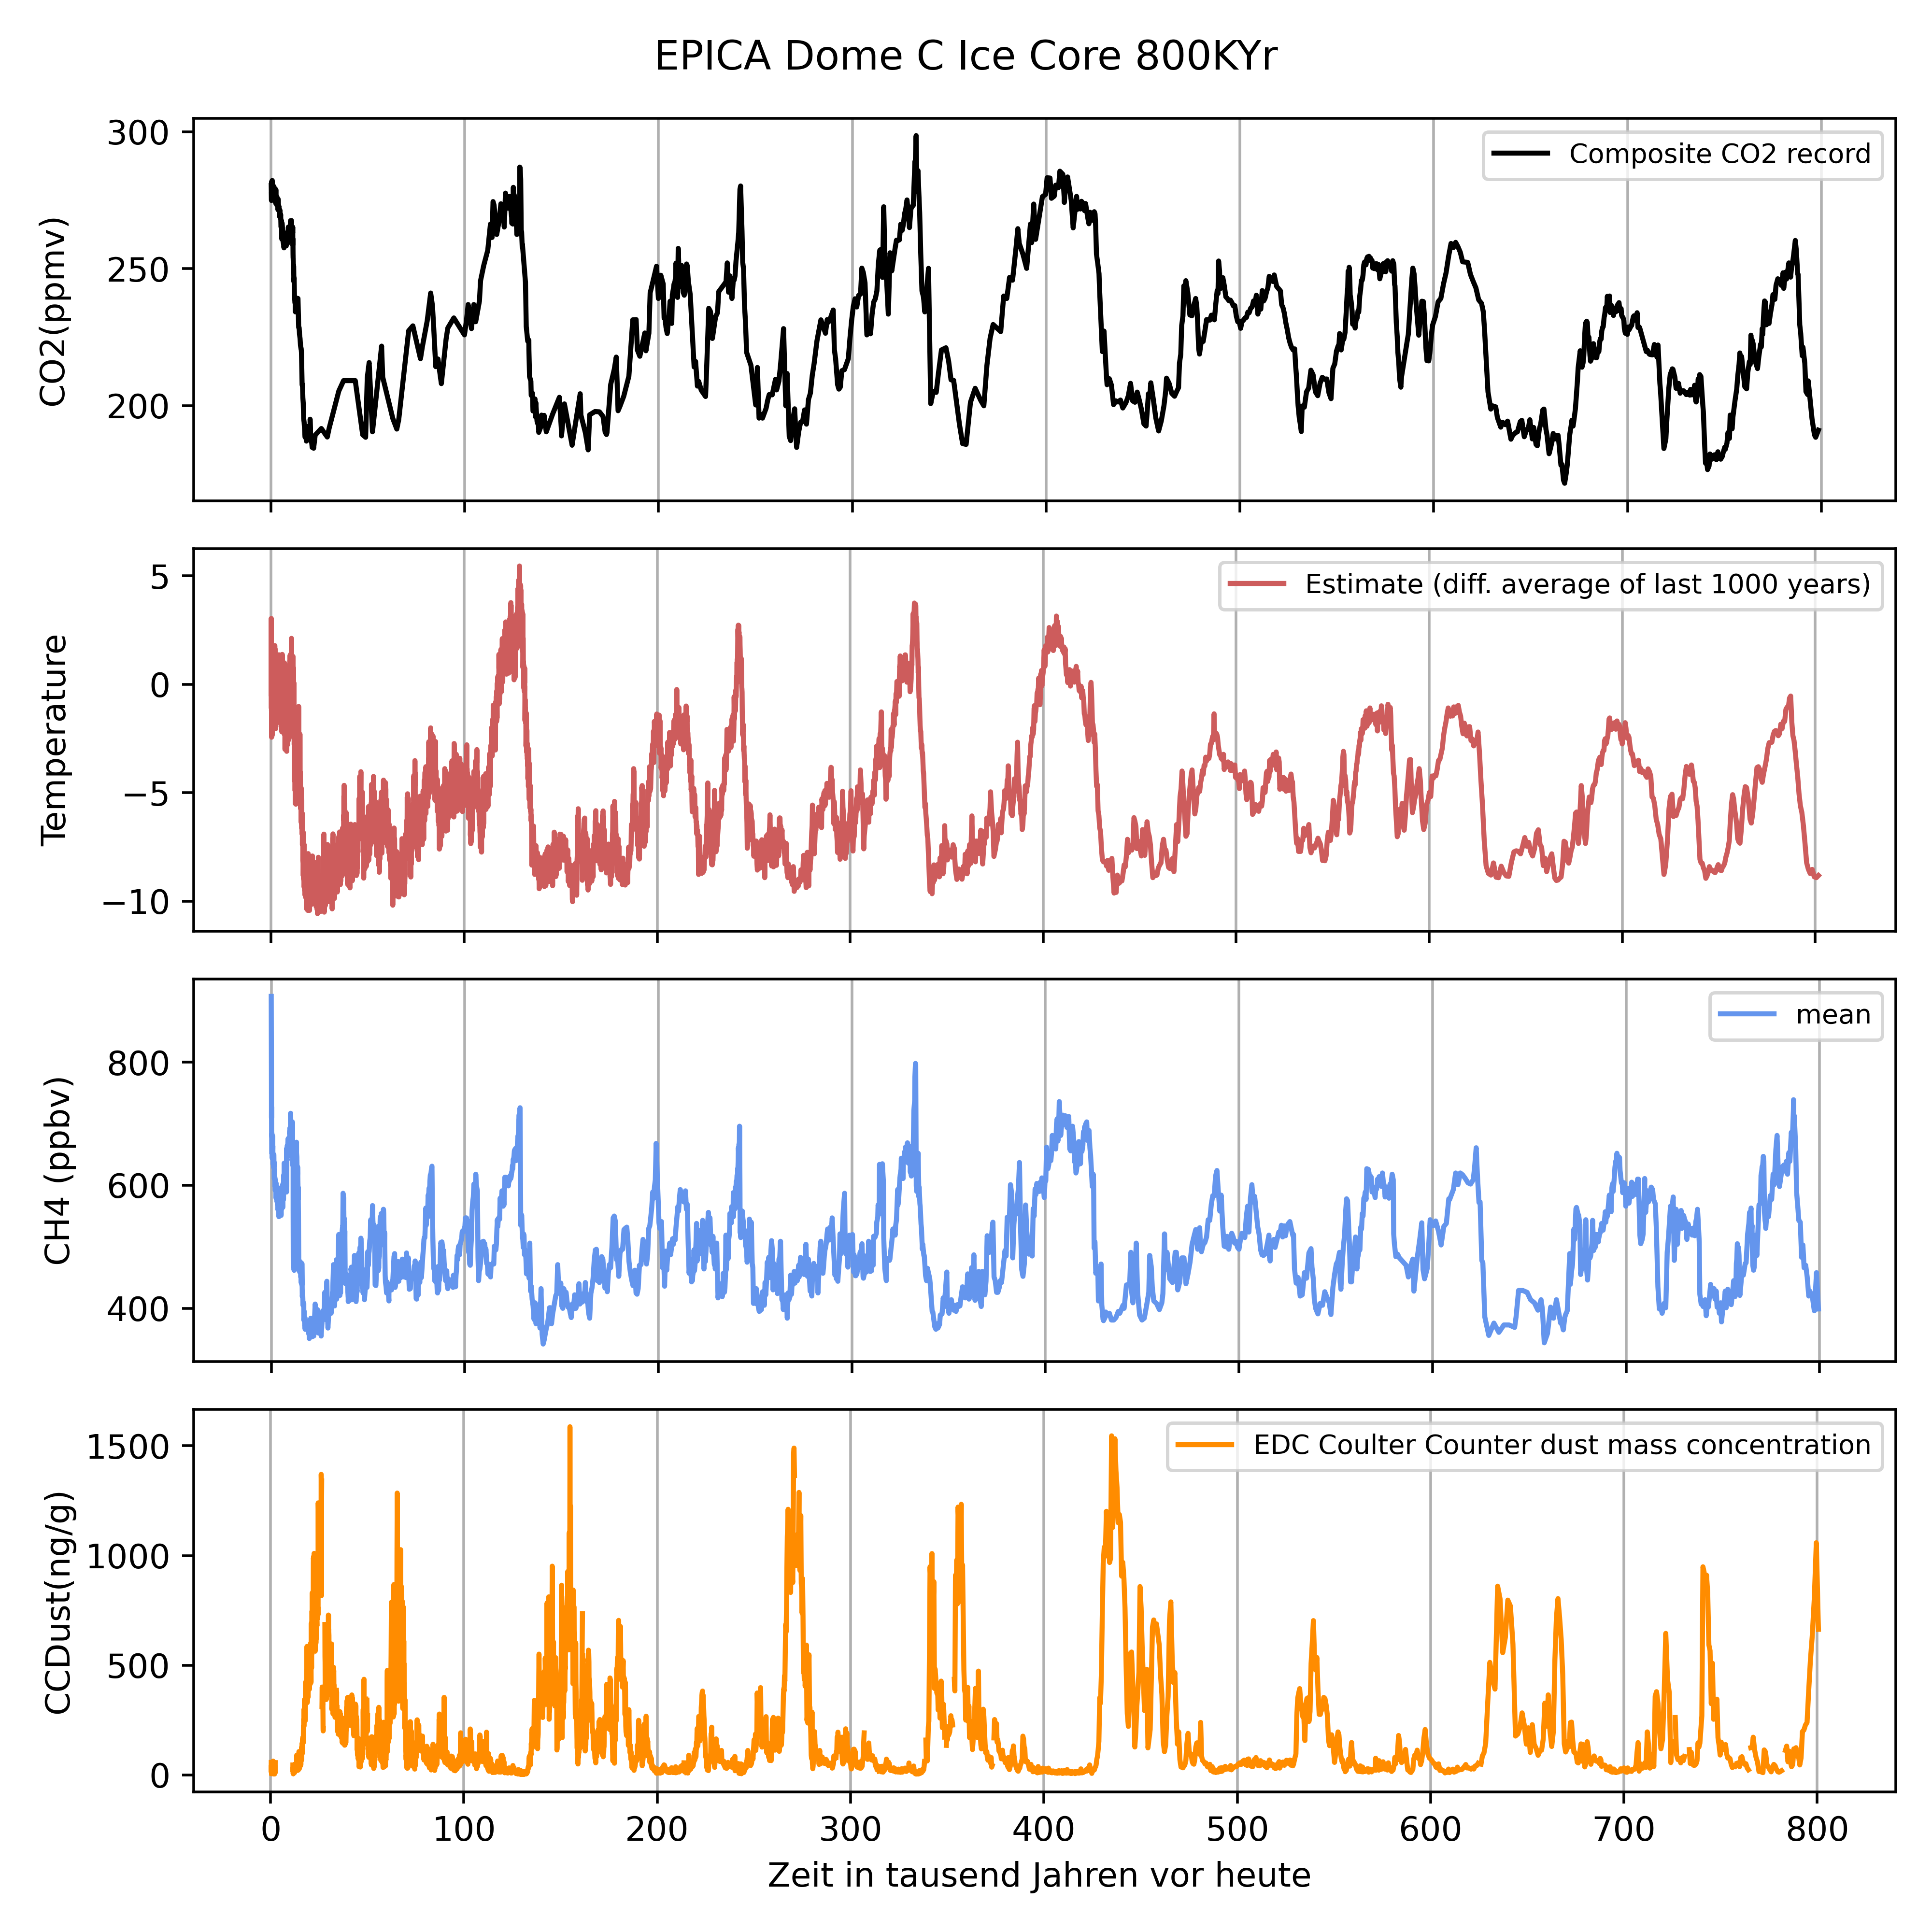
\includegraphics[width=\textwidth]{bilder/epica_icecore.png}
\caption{ Zeitreihe der letzten 800.000 Jahre für die abgeleiteten Größen \cotwo, Temperatur, Methan (CH$_4$) und Staubkonzentrationen. Erstellt aus den Datensätzen von \cite{Jouzel.2007}, \cite{Lambert.2012},\cite{Loulergue.2008},\cite{Bereiter.2015}, zur Verfügung gestellt über das \textit{National Climatic Data Center (NCDC) }  }   \label{fig:icecore}
\end{figure}

\subsection{Der südliche Ozean und die Eisenhypothese} \label{sec:Eisenhypothese}
Der Austausch von Staub und \cotwo \ hat insbesondere rund um die Antarktis eine besondere Bedeutung. Einige Modelle, die versuchen, die regelmäßigen und \textit{globalen} Klimaveränderungen im derzeitigen Eiszeitalter zu erklären, kommen damit aus, ausschließlich den südlichen Ozean zu betrachten  \citep{Fischer.2010}	. Klima und Wetter nördlich des antarktischen Kontinents werden stark durch den  Zirkumpolarstrom (ACC, Antarctic Circumpolar Current) beeinflusst. Der ACC umströmt die Landmasse zyklonal und ist gemessen an den Wassermassen die größte und für die globale Klimadynamik vermutlich wichtigste Meeresströmung überhaupt: Es wird davon ausgegangen, dass in dieser Region ein großer Teil der globalen Erwärmung umgesetzt wird. Darüber hinaus sind die Ozeane verglichen mit der Atmosphäre wahre \cotwo \ Speicher und nehmen einen Großteil (ca. 20-30 \%, vgl. \citep{IPCCpol.2019}) der anthropogenen \cotwo \ Emissionen auf, wovon schätzungsweise etwa 40 \% auf diese Region entfallen \citep{Boning.2008}.  Dies führt zu einer zunehmenden \textit{Versauerung} der Ozeane sodass der pH-Wert durch diese Entwicklung in diesem Jahrhundert weiter signifikant sinken wird \citep{IPCCpol.2019}. Der ACC verbindet Atlantik, Pazifik und den indischen Ozean miteinander, was den Austausch von Wassermassen (und die globale thermohaline Zirkulation) überhaupt erst ermöglicht. Angesichts der enormen Relevanz dieser Region scheint es plausibel, dass sämtliche Prozesse, die Einfluss auf ebendiese nehmen, auch weitreichende Implikationen für das globale Klima haben können. \\

Grundsätzlich ist der südliche Ozean ein nährstoffreiches Gebiet. Der durch den zyklonalen ACC angetriebene Ekman-Transport befördert das durch die \textit{Westerlies} initial angetriebene Oberflächenwasser nordwärts. Dieser Export wird südlich ausgeglichen, indem Wasser aus größeren Tiefen aufsteigt. Dieses an die Oberfläche beförderte Tiefenwasser ist i.d.R. nährstoffreicher als das Oberflächenwasser, da dessen Nährstoffe nicht permanent von der in der euphotischen Zone üppigeren Fauna konsumiert werden. Trotz dieses sehr effektiven Nährstofftransports sind die dortigen Konzentrationen des Phytoplanktons im Mittel geringer, als man ursprünglich erwartet hatte. Derartige Zonen mit hohem Nährstoffgehalt aber geringem Aufkommen von chlorophyllhaltigem Phytoplankton werden allgemein als HNLC (high nutrient low chlorophyll) Regionen bezeichnet. Es wurde bereits früh vermutet, dass unterschiedlicher Bedarf und Verfügbarkeit an Nährstoffen die Ursache für das gehemmte Wachstum ist. Bis heute sind diese komplexen Zusammenhänge noch nicht bis in jedes Detail verstanden (sh. Kapitel \ref{sec:Phytoplankton}). Einer dieser Nährstoffe mit besonders zahlreichen Abhängigkeiten ist Eisen. Spätestens nachdem Ende der 1980'er im Nordosten des subarktischen Pazifiks gezeigt werden konnte, dass die künstliche \textit{Düngung} von Wasserproben mit Eisen zu einem deutlichen Anstieg der Phytoplanktonproduktion führen kann, war evident, dass Eisen ein wichtiger Nährstoff für Phytoplankton ist und dessen Wachstum limitieren kann \citep{Martin.1988}. Dieser Tatbestand war nicht überraschend, da der Zusammenhang zwischen Eisen und lebenden Organismen bereits hinreichend bekannt war. Bis dahin war der Nachweis für Phytoplankton allerdings methodisch schwierig \citep{Martin.1988}. Insbesondere auf Basis dieses neuen Nachweises wird schließlich die Eisenhypothese formuliert. \\

Wie weiter oben beschrieben, übernimmt der südliche Ozean in der globalen Klimadynamik eine wichtige Rolle. Klimatische Änderungen in dieser Region korrelieren stark mit den natürlichen \cotwo -Konzentrationen der letzten 800.000 Jahre \citep{Fischer.2010}. In diesem Rahmen übt Phytoplankton direkt Einfluss aus, da im Rahmen der Photosynthese \cotwo \ konsumiert, also der Atmosphäre / dem Ozean entzogen, und dabei in organische Kohlenstoffverbindungen (Glukose) und Sauerstoff umgesetzt wird. Während dieser \textit{Wachstumsphase} werden die umgebenden \cotwo \ Konzentrationen demnach reduziert. Sorgen nun weitere Prozesse wie die \textit{Biologische Pumpe} (sh. Kapitel \ref{sec:biopump}) dafür, dass der organisch gebundene Kohlenstoff dauerhaft von der Atmosphäre separiert wird, können die \cotwo \ Konzentrationen durch erhöhte Phytoplanktonproduktionen langfristig reduziert werden. Potential für erhöhte Produktionsraten hat speziell der südliche Ozean als größte HNLC-Region. Können die überschüssigen Nährstoffe in großen Teilen dieser Region komplett durch Phytoplankton konsumiert werden, würde dies die globalen atmosphärischen \cotwo \ Konzentrationen erheblich reduzieren \citep{Martin.1990}. \citet{Martin.1990} argumentiert, dass das Wachstum von Phytoplankton im heutigen südlichen Ozean mangels biologisch verfügbarem Eisen limitiert ist. Ferner wird postuliert, dass ein nennenswerter Anteil der in Abb. \ref{fig:icecore} beschriebenen Variationen der \cotwo \ Konzentrationen zwischen Glazialen und Interglazialen aus der jeweilig unterschiedlichen Verfügbarkeit von Eisen resultiert. Der während der Glaziale höhere Staub- bzw. Eiseneintrag (sh. Abb. \ref{fig:co2iron}) soll entsprechend höhere Menge an Eisen in den Ozean eingebracht und so die Produktion von Phytoplankton verstärkt haben. Die dadurch wiederum erhöhten \textit{Archivierungsraten} von organischem Kohlenstoff hätten schließlich zu reduzierten \cotwo-Konzentrationen geführt. Entscheidend für diese Hypothese ist, dass im Gegensatz zu den meisten anderen Nährstoffen, äolischer Staub für küstenferne Gebiete als die dominante Hauptquelle von Eisen angenommen wird. Der Großteil der Hauptnährstoffe wird durch Flüsse in den Ozean eingetragen, welche die Produkte der Verwitterungsprozesse von den Landmassen abtransportieren \citep{Emerson.2009}. \citet{Tagliabue.2017} fassen zusammen, dass neben dem Eintrag von eisenhaltigen Staub inzwischen weitere Prozesse für die Verteilung des biolgisch verfügbaren Eisens (sh. Kapitel \ref{sec:Phytoplankton}) im Ozean anerkannt sind und insbesondere in höheren Breiten gegenüber dem Staubeintrag dominieren können. Neben diesem indirekten \textit{düngenden} Effekt kann Staub potentiell auch direkten Einfluss auf den Kohlenstofffluss in Richtung Tiefsee nehmen, indem Staubpartikel mit organischem Material im Oberflächenwasser aggregieren und die Sinkgeschwindigkeit damit  erhöhen \citep{vanderJagt.2018} . \\

Die Eisenhypothese wurde inzwischen in mehreren Experimenten getestet. Es konnte tatsächlich gezeigt werden, dass die Zufuhr von Eisen die Produktin steigern kann. Beispielsweise im Experiment SOIREE (Southern Ocean Iron Release Experiment) wurden Reaktionen auf die Düngung nach etwa 5 Tagen beobachtet, hauptsächlich wurde dadurch das Wachstum größerer Kieselalgen gefördert \citep{Trull.2001}. Es konnte allerdings nicht gezeigt werden, dass dadurch der Export durch die \textit{Biologische Pumpe} erhöht wurde. In vielen Regionen scheint dieser zusätzlich durch die Verfügbarkeit von Silicium limitiert. Die sogenannte \textit{Siliciumpumpe} arbeitet bereits am Limit. Obwohl geschätzt wird, dass bei etwa 40 \% des ozeanischen Oberflächenwassers Eisen ein limitierender Faktor für die Produktion von Phytoplankton sein kann \citep{Emerson.2009}, wird der Beitrag des durch äolischen Eisens (durch Staub) inzwischen geringer eingeschätzt \citep{Tagliabue.2017}. \citet{Vallelonga.2013} schätzen diesen Beitrag zur Variabilität nach dem letzten glazialen Maximum (LGM) auf maximal 20 ppmv \cotwo .

\begin{figure}[ht]
\centering
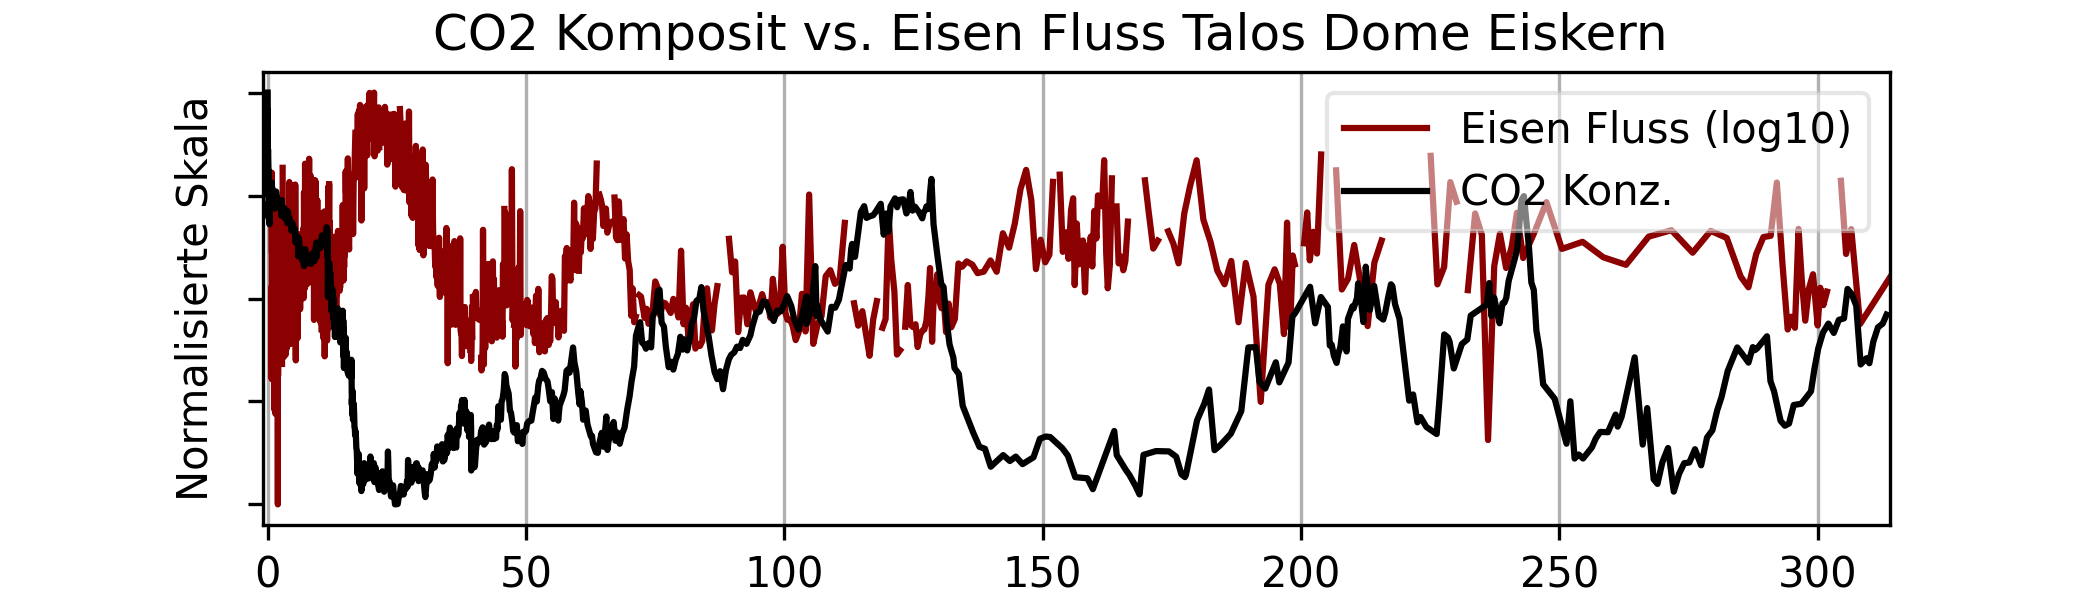
\includegraphics[width=\textwidth]{bilder/co2_iron.png}
\caption{ Zeitreihe der letzten 314.000 Jahre für die abgeleiteten Größen \cotwo (dunkelrot) und den Eisenfluss, die zur Eisenhypothese inspirierte. Die Größen weisen insbesondere während der kälteren Glaziale eine starke Antikorrelation auf. Abnehmende \cotwo -Konzentrationen gehen mit erhöhtem Eisenfluss einher. Erstellt aus den Datensätzen von \cite{Bereiter.2015} und \cite{Vallelonga.2013}, zur Verfügung gestellt über das \textit{National Climatic Data Center (NCDC) }  }   \label{fig:co2iron}
\end{figure}

\subsubsection{Wind und Oberflächenströmungen}
Verkleinerung der Tiefe der Oceanic Mixed Layer von September auf Oktober \citep{Tilburg.2002} (abchecken, dass der Bloom nicht daher kommt!). Einteilung in \textit{nördlich der Tasmanischen Front} und \textit{südlich der tasmanischen Front}? Phytoplanktonproduktion hängt von Up- und downwelling-Prozessen durch mesoskalige Wirbel ab \citep{Tilburg.2002} $\Rightarrow$ Vorticity der Ozeanströmungen berechnen?Besser sea surface height (SSH) Anonmalien angucken. Was, wenn Blüte bei \citet{Gabric.2016} aufgrund von tieferen mixed-layer aufgrund des Sturms? $\Rightarrow$ Winddaten vergleichen.

\subsection{Eigenschaften und Abhängigkeiten von Phytoplankton} \label{sec:Phytoplankton}
Bis hierhin wurde Phytoplankton bereits umfangreich erwähnt und diskutiert, tatsächlich aber noch nicht angemessen vorgestellt. Aufgrund der enormen Bedeutung sollen in diesem Abschnitt die grundsätzlichen Eigenschaften und einige der besonderen komplexen Zusammenhänge separat aufgezeigt werden. Eine seriöse Analyse der Entwicklung der Phytoplankton Konzentrationen ist ohne diese entsprechende Berücksichtigung kaum möglich.
\subsubsection{Allgemeines zu Phytoplankton} \label{sec:Phytobasics}
Durchschnittlich ungefähr 10 $\mu$g pro Liter bzw. $10^{-6}$ Prozent des Oberflächenwassers bestehen aus lebenden Organismen \citep{Emerson.2009}. Diese Konzentration ist weitaus schwächer als an Land. Die Lebenserwartung von Phytoplankton beträgt gerade einmal Stunden bis hin zu Tagen. Dieses Mikroleben entspricht aufgrund der sehr kurzen Zeitspanne in der Zusammensetzung praktisch ausschließlich dem Zustand des lokalen Ozeanwassers und kann besser durch die hinterlassenen chemischen Spuren beobachtet werden als durch direkte Untersuchung. - Phytoplankton sind Einzeller. - Die das Picophytoplankton ($<2\mu$m) in vielen Teilen des Ozeans dominierenden Cyanobakterien \textit{Synechococcus}  und \textit{Prochlorococcus} enthalten vermutlich am meisten der grünen, Licht absorbierenden Pigmente (Chlorophyll) \citep{Emerson.2009}. Kieselalgen dominieren in Regionen, wo aufsteigendes Wasser nennenswerten Einfluss nimmt, wie bspw. im südlichen Ozean. Dort besteht das Sediment größtenteils aus den \textit{Frusteln} der Kieselalgen. - Organische Meerwasser-Bestandteile werden der Größe nach in zwei verschiedene Klassen eingeteilt: feste Materie in Form von Partikeln und im Meerwasser  gelöste organische Materie. I.d.R. liegt die Grenze für die experimentelle Unterscheidung bei $0.5 \mu$m. Kleinere Partikel werden durch die Schwerebeschleunigung nur so schwach beeinflusst, dass sie (wie die tatsächlich gelöste Materie) ohne weitere Einflüsse praktisch nicht absinken. Phytoplankton liegt allerdings praktisch ausschließlich in Form von Partikeln oberhalb dieser Grenze vor \citep{Emerson.2009}.
Wachstumsbeeinflussende Faktoren sind \citep{Falkowski.1998}):
\begin{enumerate}
\item mixed-layer depth
\item nutrient fluxes
\begin{enumerate}
\item Phospor \citep{REDFIELD.1960}
\end{enumerate}
\item food-web structure
\end{enumerate}
\citet{Boyce.2010} folgern, dass der Reichtum an Phytoplankton insgesamt seit Beginn der Messungen (1899) aufgrund der Erwärmung der Ozeane abgenommen hat. Es wird geschätzt, dass das globale Median jährlich um etwa 1\% abnimmt. Da die Klimamodelle steigende (Meeres-)Temperaturen prognostizieren ist es wahrscheinlich und problematisch, dass die Menge an Phytoplankton, der Basis aller Nahrungsketten im Ozean, zukünftig noch weiter abnimmt \citep{Siegel.2010}. Klimaänderungen werden direkt (andere Ozeanchemie) und indirekt (Änderungen in der Ozeanzirkulation) die Verteilung des Phytoplanktons verändern \citep{Falkowski.1998}. Mithilfe Temperatur des Oberflächenwassers, einfallender Sonnenstrahlung, mixed-layer-depth, Up- und Downwellingzonen kann aus CHL-a Konzentration die NPP abgeleitet werden \citep{Falkowski.1998}. Für Kieselalgen ist Zufuhr von Kieselsäure essenziell; diese tritt fast ausschließlich südlich der Südpolarfront auf \citep{Falkowski.1998}.
\\\\
Vereinfacht und unter bestimmten Bedingungen besteht Phytoplankton größtenteils aus den Elementen Kohlenstoff, Stickstoff und Phospor im folgenden Verhältnis (106C/16N/1P) \citep{Falkowski.1998}. Daraus kann eine (näherungsweise, nicht allgemeingültige) Formel für die Fotosynthese abgleitet werden \citep{Emerson.2009}:
\begin{equation}
\text{106\cotwo} + \text{16HNO}_3 + \text{H}_3\text{PO}_4 + \text{122H}_2\text{O} \rightarrow \text{(CH}_2\text{O)}_{106}\text{(NH}_3\text{)}_{16}\text{H}_3\text{PO}_4 + \text{138O}_2
\end{equation}
Diese Komposition beinhaltet noch keine Spurenelemente wie Mangan, Eisen, Kobalt, Nickel, Kupfer und Zink die zwar in viel geringeren Konzentrationen auftreten, aber für das Wachstum limitierend sein können. Ein Teil dieser Metalle wird durch (mutmaßlich aus biologischen Prozessen entstandenen) Liganden komplexifiziert bzw. besetzt. Die Natur dieser Liganden ist noch nicht vollumfänglich verstanden, allerdings wird davon ausgegangen, dass ausschließlich die weiterhin \textit{freien} Metalle biologisch verfügbar sind \citep{Emerson.2009}. Berücksichtigt man die weiteren Nährstoffe, lässt sich wieder ein stöchiometrisches Verhältnis ableiten, dass an dieser Stelle wieder nicht exakt oder allgemein gilt, sondern nur die Größenordnungen der Beiträge exemplarisch aufzeigen soll \citep{Emerson.2009}:
\begin{equation}
\text{(C}_{106} \text{N}_{16} \text{P)}_{1000} \text{Fe}_8\text{Mn}_4\text{Zn}_{0.8}\text{Cu}_{0.4}\text{Co}_{0.2} \text{Cd}_{0.2}
\end{equation}
- Es wird geschätzt, dass bei etwa 40 \% des ozeanischen Oberflächenwassers Eisen ein limitierender Faktor für die Produktion von Phytoplankton sein kann \citep{Emerson.2009}, Sekundärquelle. - Eisen und andere Nährstoffe sind an der Ozeanoberfläche häufig im Vergleich zu tieferen Schichten reduziert \citep{Martin.1990}. - Andere Nährstoffe für Phytoplankton können durch aufsteigendes Tiefenwasser bereitgestellt werden. Eisen und Mangan werden hingegen hauptsächlich durch äolischen Staub eingebracht. Ansonsten sind grundsätzlich Flüsse die Hauptquelle für gelösten Eintrag von Elementen \citep{Emerson.2009} Die Konzentrationen des Elements Eisen im Meerwasser sind verglichen mit den häufigsten Stoffen wie Natrium, Chlorid, Sulfat und Magnesium sehr gering. Dennoch ist es das dritthäufigste Element in marinen Sedimenten. \citep{Emerson.2009} - Verweildauer von etwa 6 Monaten in oberflächennahem Wasser bis ca. 150m Tiefe \citep{Hayes.2015}. Nitrogenase (Enzymkomplex) kann N$_2$ reduzieren und Stickstoff somit biologisch verfügbar machen. Laut \citet{Emerson.2009} ist dies das extremste Beispiel, für die Limitierung durch Eisen, da diese Enzyme zu einem großen Teil aus Eisen bestehen. Nitrogenase selbst benötigt (bzw. besteht aus) Eisen. Meistens Trichdesmiumspp., das N$_2$ bindet \citep{Falkowski.1998}.  In nährstoffarmen Gewässern haben extrem kleine Phytoplankton-Organisamen bei der Verarbeitung von Nährstoffen (Exkrementen der Verbraucher) einen Wettbewerbsvorteil, da großes Oberflächen zu Volumen- Verhältnis \citep{Falkowski.1998}.Wenn hingegen \textit{neue} Nährstoffe bspw. durch Upwelling nach oben gelangen, hat größeres Phytoplankton, insbesondere Kieselalgen einen Wettbewerbsvorteil (aufgrund Vakuole, schnellere Aufahme). -Dementsprechend wurde beobachtet, dass in mit löslichem Eisen \textit{gedüngten} Arealen  Kieselalgen im Vergleich zu anderem Phytoplankton besonders stark reagieren, also wachsen. Die Zugabe von Eisen fördert, dass Nitrate (NO$_3^-$) zu Ammonium-Ionen (NH$_4^+$) reduziert werden, welche bei der Fotosynthese von Plankton mit hohem Bedarf an Nitraten besonders schnell verwendet werden können.  \citep{Emerson.2009}. -Das Plankton, das sich wiederum von diesen ernährt, ist typischerweise größer, benötigt für Entwicklung (Larvenstadium) mehr Zeit; dadurch im gegensatz zu obigen Arealen Blooms möglich und stärkere biologische Pumpe.
\\\\ Insbesondere im südlichen Ozean kann auch Mangan limitierender Faktor sein \citep{Browning.2021}. Bisher wurde Mangan diesbezüglich nicht verdächtigt. Die Besonderheit bei Mangan ist, dass dieses Spurenmetall im Gegensatz zu Eisen kaum durch Liganden besetzt wird und damit wesentlich mehr biologisch verfügbar ist \citep{Emerson.2009}. Untersuchungen von Eisbohrkernen zeigen, dass Eisenzufuhr durch äolischen Staub in glazialen Perioden um eine Größenordnung größer war als in Interglazialen \citep{Falkowski.1998}. - Es gab großskalige Experimente, in denen in Phosphor- und Nitratreichen Gewässern Eisen hinzugefügt wurde \citep{Emerson.2009}. -
\subsubsection{Biologische Pumpe} \label{sec:biopump}
- Der Export von organischer Materie aus der euphotischen Zone ist für den Hauptteil der chemischen Prozesse in der Tiefsee verantwortlich \citep{Emerson.2009}. - Niedriger Sauerstoffgehalt in der Tiefsee weist auf starke biologische Pumpe hin (dortige durch mehr absinkendes Plankton angereicherte Organismen verbrauchen mehr Sauerstoff?). Im aktuellen Ozean beträgt der (Sink)Fluss ca. 16 Pg Kohlenstoff pro Jahr \citep{Falkowski.1998} (laut \citet{Emerson.2009} Größenordnung 5  Pg??). In Küstengebieten (Upwelling) sehr deutlich $\Rightarrow$ Fischerei profitiert. Hoher Sauerstoffgehalt führt zu oxidiertem Eisen; oxidiertes Eisen ist nicht löslich und sinkt $\Rightarrow$ geringer Eisengehalt \citep{Falkowski.1998}. Es wird angenommen , dass die Leistung der biologischen Pumpe aufgrund der Klimaveränderungen insgesamt global abnehmen wird. - Aufgrund der höheren Dichte von Mineralen ( vereinfachend angenommen ca. $2.5$ g cm$^{-3}$) im Gegensatz zu organischer Materie (ca. $1.1$ g cm$^{-3}$)  und Meerwasser (ca. $1$ g cm$^{-3}$) kann abgeschätzt werden, dass anorganische Partikel etwa 15 mal schneller sinken als rein organische. Entsprechend kann abgeleitet werden, dass Organismen ohne zusätzlichen mineralischen Ballast aufgrund der geringen Sinkgeschwindigkeit die euphotische Zone praktisch kaum verlassen können. Zusätzlich bietet eine mineralische Hülle entsprechenden Schutz vor Oxidation der organischen Materie, die ansonsten bereits innerhalb der ersten 2000m während des Sinkens einsetzen würde\citep{Emerson.2009}.
\subsubsection{Düngung funktioniert nicht}
verschiedene Ursachen. Verweilzeit in Oberflächenwasser \citep{Hayes.2015}. Aufnahmefähigkeit / Rezeptivität ist saisonal variabel \citep{Gabric.2016}, Sekundärquelle.\citep{Falkowski.1998}. Zeitreihen für Messungen der Ozeanbiologie sind im Vergleich zu Land sehr kurz, wodurch Schätzen auch unzuverlässiger sein können \citep{Falkowski.1998}. Häufigste Beschränkung ist durch Verfügbarkeit von gebundenem anorganischem Stickstoff \citep{Falkowski.1998}. Daneben wurde aber auch für viele weitere Metalle wie Ni, Zn, Co, Cd, Cu ein messbarer Einfluss auf die Phytoplanktonproduktion bzw. die dafür erforderlichen Enzyme beobachtet.
\subsection{Staub in Australien} \label{sec:Staub}
Wichtige Verbindung zu Energie- und Kohlenstoffkreislauf \citep{Shao.2011} - Staub entstammt nicht nur ariden Wüstengebieten. Ein nennenswerter Anteil ($>$ 5\%) entsteht in kalten/glazialen Regionen hauptsächlich durch die Bewegungen von Gletschermassen und den damit verbundenen Abreibungen. Verwitterungsprozesse spielen im Gegensatz zu ariden Gebieten eine untergeordnete Rolle \citep{Marx.2018}. -
\subsubsection{Staubquellen in Australien}
Staub, der durch entsprechende Quellen emittiert wird, entstammt häufig einem anderen Ort. Dies sind i.d.R. benachbarte Regionen höherer Feuchte, in denen chemische und physikalische Verwitterung stattfindet. Während des Transports zur Region der Emission wird die Partikelgröße weiter reduziert (zermahlen, Separation durch Wind). Dementsprechend kann die Verfügbarkeit von Staub paradoxerweise von einem ausreichend hohen (Feuchte)Fluss in die Region abhängen. Dies trifft insbesondere auf die endorheischen Systeme rund um das Lakre Eyre Becken in Australien zu \citep{Marx.2018}. - größte Teil Zentralaustralien \citep{Shao.2011} siehe auch Lake Eyre basin. \\\\
Laut \citet{Deckker.2019} sind \textit{Kati Thanda-Lake Eyre} Region und \textit{Darling Riverine Plain} (Oberlauf des Darling River) Hauptquellen. Der Kontinent deckt insgesamt ein breites Spektrum an Oberflächengeologie ab, sehr alte Landmasse; einige Flächen sind mehr als 2.5 Milliarden Jahre alt (aus dem Archean). Durch die Besiedelung und Landnutzung durch den Menschen haben sich signifikante Änderungen ergeben, die bis 1945 mutmaßlich zu einer höheren Frequenz an Staubstürmen geführt haben. Nach verbesserter Landnutzung nahmen auch die Staubstürme wieder ab \citep{Deckker.2019}. Vgl. größte Staubereignisse vor 2009 waren in den 1940'ern.
\subsubsection{Eisen in Staub}
Nicht jede Form von Eisen kann als Dünger dienen. Muss entsprechend gelöstes (?) Eisen sein. Transportprozesse und Wolkenbildungen können die Transformation zu diesem tauglichen Eisen fördern \citep{Shao.2011}. Die Planktonart Trichodesmium kann die Rate des Eisenauflösens von Oxiden und Staub beschleunigen (im Gegensatz zu anderem Phytoplankton) \citep{Gabric.2016}. In Sediment enthält Staub häufig die Fe$^{3+}$ Minerale Hämatit und Goethit \citep{Reynolds.2014}. Die Ergebnisse von \citet{Reynolds.2014} legen nahe, dass der Eisengehalt (Magnetit) des Staubes beim \textit{Red-Dawn} durch die dichten urbanen Gebiete an der Küste weiter erhöht wurde.
\begin{table}[H]
\begin{tabularx}{\textwidth}{X X l}
		\toprule
			\thead{Eisenoxid(hydrate)} & \thead{Verhältnisformel} &  \thead{Vorkommen} \\
		\midrule
		Hämatit & Fe$_2$O$_3$ & Mineral, trigonales Kristallsystem \\
		Maghemit & Fe$_2$O$_3$ & Mineral, kubisches Kristallsystem \\
		Magnetit & Fe$_2$O$_4$ & Mineral, kubisches Kristallsystem \\
		Goethit & $\alpha$-Fe$^{3+}$O(OH) & Mineral, orthorhombisches Kristallsystem \\
		\bottomrule
\end{tabularx}
\caption{Beschreibung} \label{table:eisenoxid}
\end{table}

\subsubsection{Deposition}
Hauptursache für die Deposition/Ablagerung von weit transportiertem Staub ist das \textit{Auswaschen} durch Regen \citep{Marx.2018}, Sekundärquelle. -


\subsubsection{Beschreibung des Staubsturms in September 2009} \label{sec:reddawn}
stärkstes (in Bezug auf Sichtweitenreduzierung) Staubevent über Sydney seit es verlässliche Aufzeichnungen gibt (1940, \citet{Leys.2011}). Staubstürme üblich im ariden Inland. Vorangegangen sind Monate und Jahre mit im Vergleich zum Durchschnitt höheren Temperaturen und unterdurchschnittlichem Niederschlag; dadurch schwache Vegetation und trockene Erdböden \citep{Leys.2011}. Aufgrund der hohen Intensität wird dieser Zeitraum \textit{Millenium Drought} getauft \citep{Deckker.2014}, Sekundärquelle.

\subsubsection{Staubtransport}
Wird Staub über mehrere tausend Kilometer transportiert, verleiben i.d.R. nur Staubpartikel mit Größen von $<$20$\mu$m \citep{Marx.2018}, Sekundärquelle.

\section{Methoden und Daten} \label{sec:Methoden}
Um testen zu können, ob ein extremes Staubereignis Auswirkungen auf die Phytoplanktonproduktion in einer bestimmten Region hat, ist eine geeignete Datenbasis erforderlich. Grundsätzlich müssen hierzu zwei Variablen räumlich und zeitlich quantifiziert werden: Staub- und Phytoplankton-Konzentrationen. In beiden Fällen ist die Auflösung in jeder dieser Dimensionen stark beschränkt. Speziell Ausdehnung und Trajektorien von Staubstürmen müssen aufgrund der spärlichen Beobachtungsdaten (siehe Kapitel  \ref{sec:reddawn}) größtenteils geschätzt werden. Simulationen leistungsfähiger Modelle können die Auswertungen deutlich verbessern. In Rahmen dieser Arbeit wird eine spezielle WRF-Simulation (sh. Kapitel \ref{sec:wrf}) verwendet, um genauere Aussagen über das Verhalten der Staubwolke treffen zu können. Die Konzentrationen des Phytoplanktons werden (wie üblich) aus satellitengestützten täglichen Messungen der Chlorophyll a Konzentrationen abgeleitet (sh. Kapitel \ref{sec:chla}). Für den finalen Test eines möglichen Zusammenhangs werden die in Kapitel \ref{sec:stats} vorgestellten statistischen Methoden angewendet.

\subsection{WRF Modell} \label{sec:wrf}
Das \textit{Weather Research and Forecasting} (WRF) Modell ist ein mesoskaliges System zur numerischen Wettersimulation. Es findet in der Atmosphärenforschung breite Anwendung und kann für verschiedene Zwecke mit Auflösungen von weniger als einem Meter bis hin zu mehreren tausend Kilometern eingesetzt werden \citep{NCAR.2021}. Das ursprüngliche Modelle wurde um ein Modul ergänzt, dass neben den \textit{üblichen} meteorologischen Größen auch Staub-Emission, -Transport und -Deposition berücksichtigt. Im Rahmen dieser Arbeit wird der Output eines WRF-Modells der Version 4.1.2 verwendet, welcher zusätzlich die modellierten Konzentrationen des Elements Eisen enthält. Als Staub-Emissionsschema wurde jenes von \citet{Shao.2004} verwendet. Das Modell berechnet die Staubkonzentrationen für 5 verschiedene Korngrößenklassen, welche in Tabelle \ref{table:wrf} dargestellt sind. Simuliert wurde der Zeitraum vom 18.09.2009 um 0 Uhr UTC bis zum 30.09.2009 um 0 Uhr UTC. Die verfügbaren Variablen werden in der Ausgabedatei in einem Intervall von drei Stunden gespeichert, wodurch sich insgesamt 97 auswertbare Zeitschritte ergeben. Zum Startzeitpunkt werden dem Modell keine atmosphärischen Staubkonzentrationen übergeben. Etwaige Emissionen zu früheren Zeitpunkten werden demnach vernachlässigt. Räumlich deckt das Modell von 110.3° Ost bis 170.3° West und von 57.06° S bis 9.89° S den gesamten australischen Kontinent, das tasmanische Meer, Neuseeland und Teile des südlichen Ozeans und Pazifiks ab. Dieses Gebiet wird mit 164$\times$124 (Ost-West$\times$Süd-Nord) Gitterpunkten abgedeckt. Ein Gitterpunkt repräsentiert damit ein Gebiet von etwa 53.3 km$\times$29.5 km (am nördlichsten Punkt in der Domäne, im Süden sind es 29.4 km$\times$53.3 km). Mehrere Größen, die für Emission, Transport und Deposition wichtig sind (bspw. lokale Form des Geländes, steile Topographie, Rauheit, Turbulenzen), können nicht aufgelöst werden und müssen im Modell parametrisiert werden. Die vertikale Verteilung wird auf 32 Höhenlevel simuliert. Das unterste Höhenlevel ist (entsprechend der Auflösung) geländefolgend, das oberste liegt oberhalb der Troposphäre zwischen 19.044 m und 20.230 m über Meeresniveau.
\begin{table}[H]
\begin{tabularx}{0.3\textwidth}{X X}
		\toprule
			\thead{Größenklasse} & \thead{Effektiver Radius}\\
		\midrule
		1 & $0.5 \ \mu$m \\
		2 & $1.4 \ \mu$m \\
		3 & $2.4 \ \mu$m  \\
		4 & $4.5 \ \mu$m \\
		5 & $8.0 \ \mu$m  \\
		\bottomrule
\end{tabularx}
\caption{Die Staubpartikel wurden in verschiedene Korngrößen unterteilt} \label{table:wrf}
\end{table}
\subsubsection{Emissions Schema}
Zur Modellierung der Staubemissionen wurde das Schema von \citet{Shao.2004} verwendet und in WRF implementiert. Als Auslöser für Emissionen werden grundsätzlich zwei Mechanismen erwogen: Beschuss durch Salz und der Zerfall von Aggregaten. Zusammengefasst setzt sich das Emissionsschema \citep{Shao.2004} aus folgenden Gleichungen zusammen:
\begin{align}
\tilde{F} (d_i,d_s) &= c_y \eta_{fi} \left[\left(1-\gamma\right) + \gamma
\sigma_p \right] \left(1+\sigma_m \right) \frac{g \cdot Q}{u^2_*} \\
\gamma &= \exp \left[-\left(u_* - u_{*t} \right)^3\right] \\
\sigma_m &= 12 \cdot u_*^2 \frac{\rho_b}{p} \left(1 +14 \cdot u_* \sqrt{\frac{\rho_b}{p}} \right)
\end{align}
Dabei ist $\tilde{F}(d_i,d_s)$ die Emissionsrate für die Staubpartikelgröße $d_i$ und das Salz der Partikelgröße $d_s$; $c_y$ ein dimensionsloser Koeffizient; $\eta_{fi}$ der Anteil des insgesamt emittierbaren Staubs; $\sigma_p = \frac{\eta_{mi}}{\eta_{fi}} = \frac{p_{m}(d_i)}{p_{f}(d_i)}$ das Verhältnis zwischen der Massenverteilung freien Staubs $\eta_{mi}$ zu der des ingesamt emissionsfähigen Staubs $\eta_{fi}$ pro Einheitsbodenmasse für die Partikelgrößenklasse $i$ bzw. den entsprechenden Verteilungen für die Partikelgrößenverteilungen $p_{m}(d_i)$ und $p_{f}(d_i)$;  $\sigma_m= \frac{m_\Omega}{m}$ das Verhältnis zwischen der Masse  $m$ des einschlagenden Partikels und der durch \textit{Bombardement} ausgeworfenen Masse $m_\Omega$; $g$ die Erdschwerebeschleunigung; $Q$ der stromweise Salzfluss; $u_*^2$ die Reibungsgeschwindigkeit; $u_{*t}^2$ der Schwellenwert für die Reibungsgeschwindigkeit; $\rho_b$ die Bodenschüttdichte und $p$ der plastische Bodendruck.
\subsection{Chlorophyll a} \label{sec:chla}
Um die Taxonomie und die genauen Konzentrationen des Phytoplanktons im Meerwasser abzuleiten, sind in situ Messungen erforderlich. Für die Untersuchung eines Zusammenhangs in dieser Arbeit ist es allerdings ausreichend, die grundsätzliche Tendenz der Entwicklung der Phytoplankton Konzentrationen zu quantifizieren. Eine explizite Kenntnis der speziellen Zusammensetzung ist nicht erforderlich, kann aber anhand vorangegangener Untersuchungen und der für die jeweilige Region erwartbaren Verteilungen abgeschätzt werden. Messungen des in Pflanzen enthaltenen Farbstoffs Chlorophyll erlauben, Produktion und Konzentrationen von Phytoplankton abzuleiten \citep{RYTHER.1957}. Dementsprechend ist es zu diesem Zweck üblich, die Nettoprimärproduktion aus Satellitenbildern abzuleiten, welchen Werte des Hauptpigments \textit{Chlorophyll a} zugewiesen werden können. Da die Reaktionszeit auf möglichen \textit{Dünger} mit 4-5 Tagen (vgl. Kapitel \ref{sec:Phytobasics}) relativ kurz ist, ist es vorteilhaft, zeitlich möglichst hoch aufgelöste, tägliche Daten zu verwenden. Eine erhebliche Einschränkung dieser satellitengestützten Daten ist, dass die Beobachtungen nur über eis- und wolkenfreiem Himmel möglich sind. Zusätzlich kann reflektiertes Sonnenlicht die Ableitung erschweren. Auf Abbildung \ref{fig:chla} wird beispielhaft demonstriert, dass diese Faktoren zu einer sehr schlechten räumlichen Auflösung führen können. Glücklicherweise bietet der \textit{Copernicus Marine Service} bzw. \citet{Saulquin.2019} einen überarbeiteten Datensatz für den Betrachtungszeitraum, welcher die fehlenden Beobachtungsdaten mithilfe aktueller Algorithmen in täglicher Auflösung interpoliert. Obwohl dieser Datensatz die gewässertypischen Besonderheiten berücksichtigt und auf Basis fundierter Interpolationsmethoden zusammengestellt wurde, muss aufgrund der schlechten Abdeckung (insbesondere mit zunehmender geographischer Breite) bei der späteren Interpretation ein entsprechend hoher möglicher Fehler beachtet werden. Die Werte werden  aus den Messungen mehrerer Sensoren/Spektrometer (MERIS, MODIS und SeaWiFS) zusammengestellt.

\begin{figure}[ht]
	\begin{minipage}[c]{0.49\textwidth}
		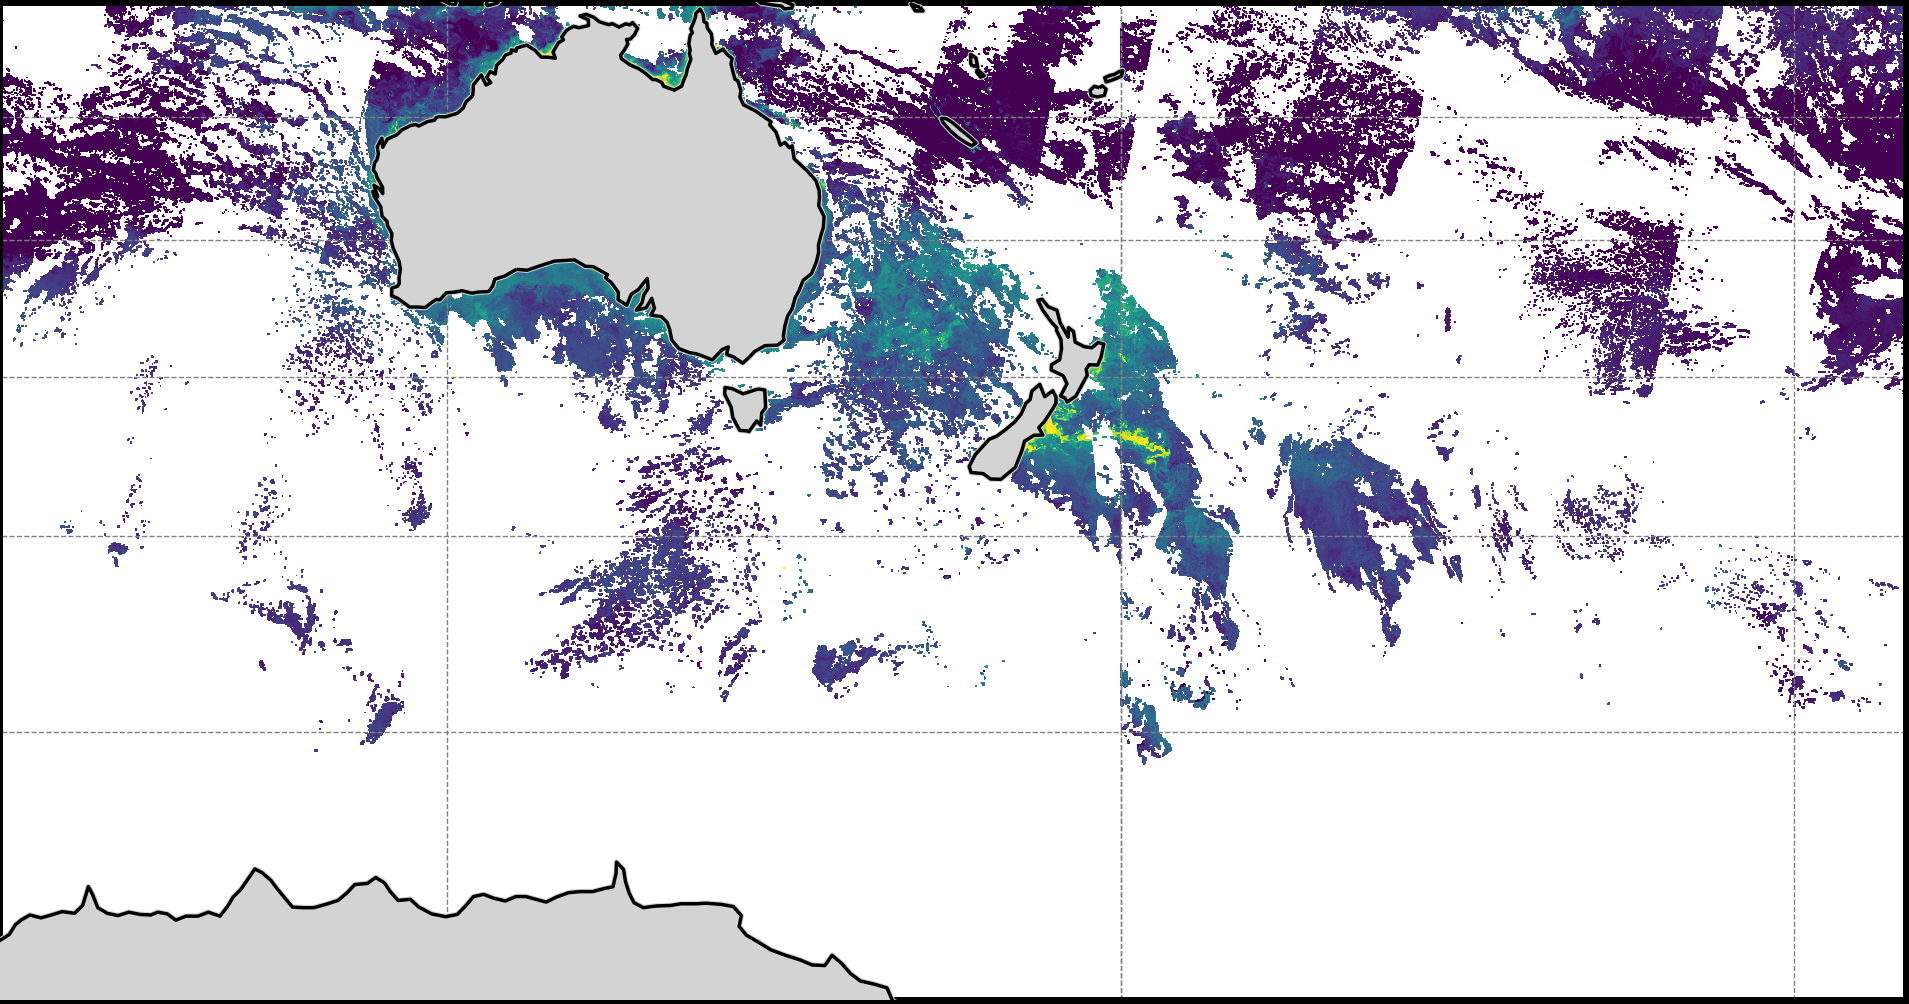
\includegraphics[width=\textwidth]{bilder/chla_raw.png}
	\end{minipage}\hfill
	\begin{minipage}[c]{0.49\textwidth}
		 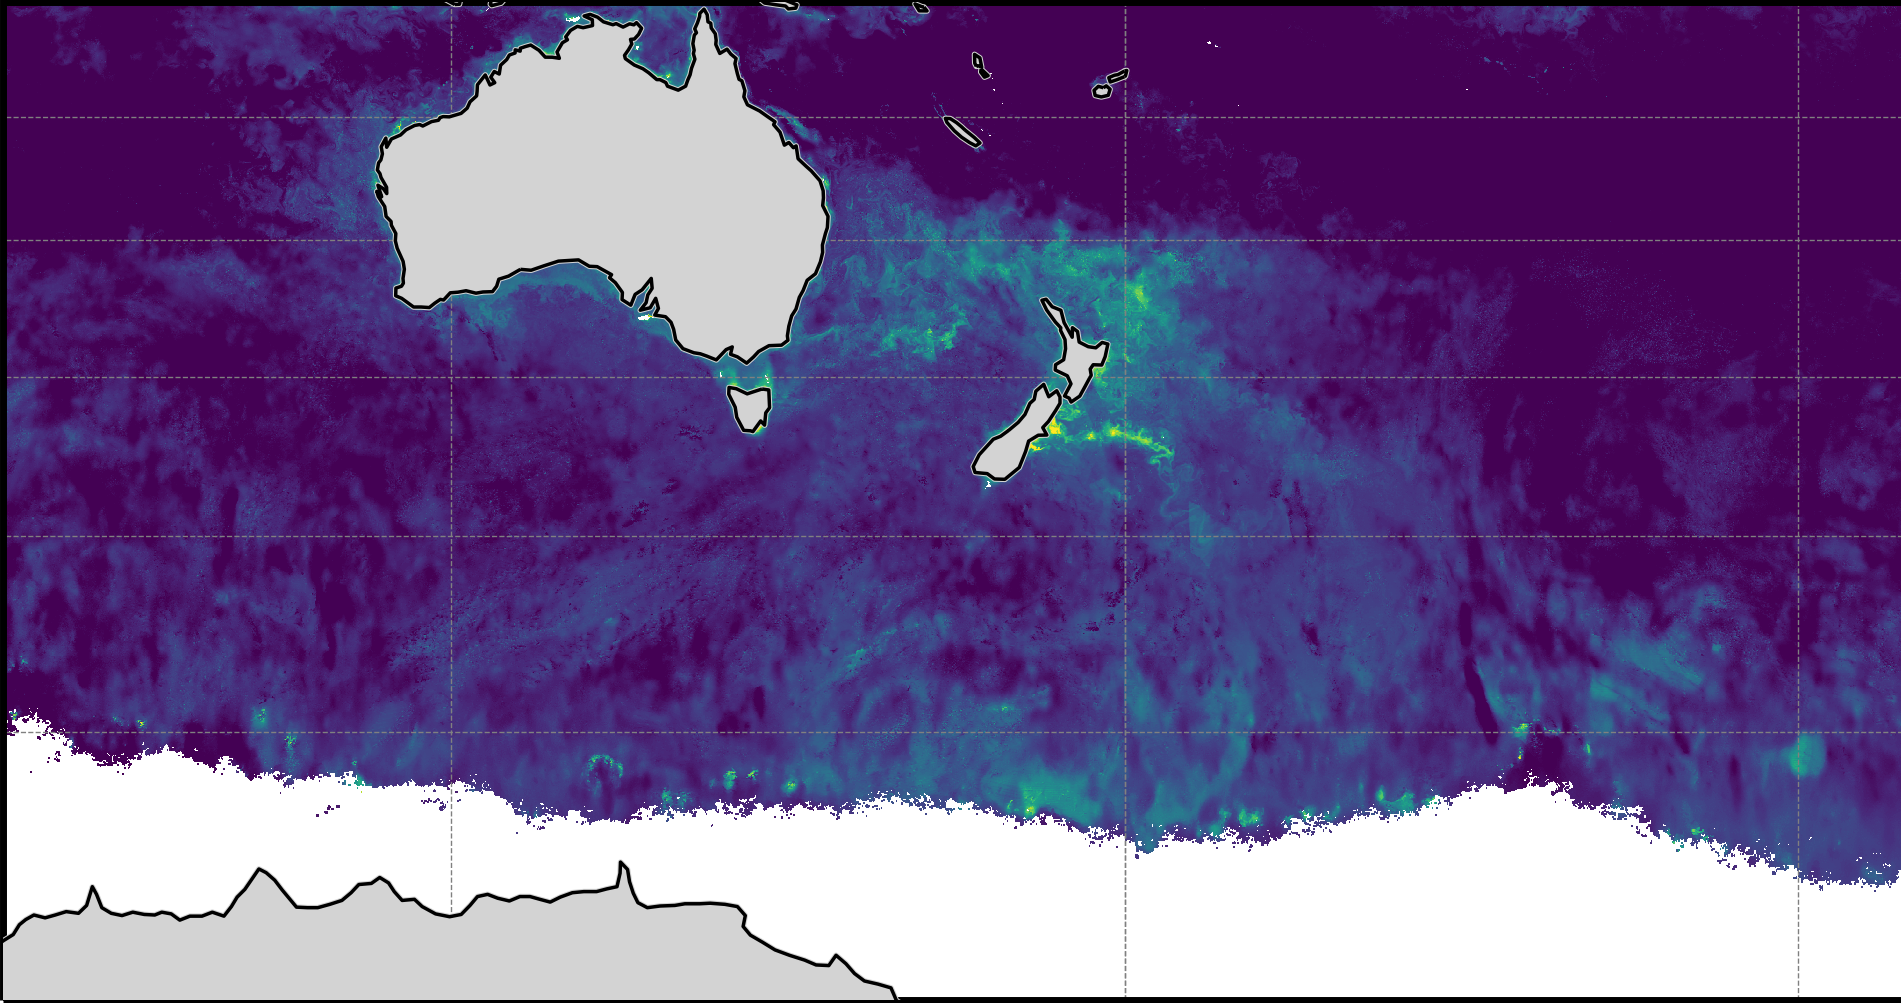
\includegraphics[width=\textwidth]{bilder/chla_interpol.png}
	\end{minipage}\hfill
	\caption{Beispielhaft die zum 01.09.2009 abgeleiteten Chlorophyll a Konzentrationen. Links: Ableitung auf Basis der Beobachtungsdaten (Ocean colour daily data des Climate Data Store). Für alle weißen Flächen liegen keine Daten vor. Rechts: Mithilfe weiterer Algorithmen von \citet{Saulquin.2019} interpolierte Werte für eine vollständigere Abdeckung.} \label{fig:chla}
\end{figure}

\subsection{Modell für den Hypothesentest} \label{sec:hypotest}
Wie in den vorangegangenen Kapiteln aufgezeigt wurde, können verschiedenste Faktoren dazu führen, dass trotz des gemeinhin bekannten \textit{düngenden} Effektes von Eisen auf Phytoplankton kein Zusammenhang zum Staubsturm in Form des erhöhten Eintrags von Staub bzw. Eisen in den Ozean beobachtet werden kann. Im Rahmen dieser Arbeit soll die einfache Hypothese getestet werden, dass eine mögliche Reaktion des Phytoplanktons vordergründig dadurch limitiert ist, dass die eingetragenen Nährstoffe, insbesondere Eisen, nicht ausreichend lange im Oberflächenwasser verweilen um von den Organismen konsumiert zu werden. Aufgrund der vergleichsweise hohen Sinkgeschwindigkeit des Formats, in dem Eisen hauptsächlich eingetragen wird, entzieht sich dieser Nährstoff der euphotischen Zone. Um diese Hypothese zu testen, werden vereinfachende Annahmen zur Reaktionszeit des Phytoplanktons $T_{Phy}$, der Sinkgeschwindigkeit $v_i$ der jeweiligen Korngröße $i$ , der Tiefe der aktiven euphotischen Zone (bzw. MLD) $h$ und der damit verbundenen Verweilzeit $T_{i}$ der zusätzlichen Nährstoffe gemacht. In Regionen, in denen die Verweilzeit $T_{i}$ größer als die Reaktionszeit $T_{Phy}$ ist, sollten unter der Annahme sonst unveränderter Bedingungen Reaktionen beobachtet werden können. Da der Staub nicht nur einmalig zu einem bestimmten Zeitpunkt eingetragen wird, sondern an unterschiedlichen Orten über unterschiedliche Zeiträume, ist es erforderlich, für jeden Modellpunkt ein Budget zu betrachten. Der Hypothese folgend können Orte mit kontinuierlichem Eintrag über einen längeren Zeitraum eine stärkere Reaktion zeigen. Diese Lokationen sollen mithilfe der WRF-Simulation identifiziert und anschließend mit den Chlorphyll a Daten verglichen werden. Um auszuschließen, dass die Reaktionen aus einem anderen, vom Staubsturm unabhängigen, Faktor resultieren, sollten diese über der Standardabweichung des klimatischen Mittels liegen.
Sigmoidfunktion zur Aktivierung:
\begin{equation}
\text{sig}(x) = \frac{1}{1+e^{-x}} = \frac{1}{2} \cdot \left(1 + \tanh \frac{x}{2} \right)
\end{equation}
\begin{align}
R(t) &= \sum\limits_{i=1}^5 \text{sig} ( T_{i} - T_{Phy}) \\
&= \sum\limits_{i=1}^5 \text{sig} (\frac{h}{v_i} - T_{Phy})
\end{align}

\subsubsection{Evaluierung der Parameter}
Zur Berechnung der Sinkgeschwindigkeit Stokes?
turn-over time ist von Größenordnung einer Woche oder weniger \citep{Falkowski.1998}: abgeleitet durch: 45 bis 50 Pg Kohlenstoff produzieren Phytoplankton pro Jahr, aktuell im Ozean sind aber immer nur ca. 1 Pg, das heißt dass das jeweils aktuelle Phytoplankton immer nach ca. einer Woche \textit{umgesetzt} wurde. Die Proben von \citet{Martin.1988} zeigten an Tag 4 des Experiments eine signifikante Reaktion auf die Zugabe von Eisen (im Vergleich zu den unbehandelten Kontrollen).



\section{Gabric.2016}

\begin{itemize}
\item Tasman Sea $25^\circ$ S bis $40^\circ$ S Untersuchungsareal
\item data: Chl + aeorosol optical depth (AOD)
\begin{itemize}
\item chl data: daily + 8 day MODIS-AQUA
\item AOD data: 550 nm, 4km resolution
\end{itemize}
\item divided into $5^\circ$ lattitude band
\item DVR kumulativ
\item Hovmoller Plots (x: zeit, y: latidude, longitude)
\item cloud processing / wet deposition wichtig
\item Response hauptsächlich südlich der tasmanischen Front ($\approx 32^\circ$ S)
\item Staubdeposition weiter im Norden
\end{itemize}



\subsection{Der südliche Ozean}
Schätzungsweise 45-62 \% der gesamten Wärmezunahme zwischen 2005 und 2017 in den oberen 2000m des globalen Ozeans entfielen auf den südlichen Ozean \citep{IPCCpol.2019}. Auch im tiefen Ozean $>2000m$ fand wahrscheinlich eine Erwärmung statt. Zusammen mit dem steigenden Eintrag von Süßwasser durch abschmelzende Eisschilde führt diese Erwärmung zu  einer zunehmenden Stratifizierung der oberen Ozeanschichten. Durch diese höhere hydrodynamische Stabilität wird  der Austausch von Nährstoffen in lichtdurchflutete Schichten erschwert, sodass die dortige Produktion von Phytoplankton beeinträchtigt ist. In der Arktis führten die Veränderungen in der Eisbedeckung zu einer erhöhten Nettoprimärproduktion, Phytoplankton-Blüten treten früher im Jahr auf. Rund um die Antarktis kann dies allerdings nicht pauschal beobachtet werden \citep{IPCCpol.2019}. Allerdings wird eine Südwärtsverlagerung des antarktischen Krillvorkommens vermutet. Derzeitige Klimaprognosen deuten daraufhin, dass die Nettoprimärproduktion in Arktis und Antarktis erhöhen , aber gleichzeitig in tropischen Gewässer deutlich sinken wird. Grundsätzlich bietet der südliche bzw. antarktische Ozean ein hohes Potential für die Produktion von Phytoplankton. Im (südhemisphärischen) Sommer sind große Teile der oberen Ozeanschichten ausreichend lichtdurchflutet und Nährstoffe (mit Ausnahme von löslichem Eisen) können durch das allgemeine Aufströmen aus der Tiefe an die Oberfläche transportiert werden \citep{Martin.1990}. -  Der antarkische Zirkumpolarstrom kann je nach Zone verschiedene chemikalische Eigenschaften aufweisen:

\begin{enumerate}
\item Subtropische Front
\item Subantarktische Zone
\item Subantarktische Front
\item polare Frontzone
\item Polarfront
\item Antarktische Zone
\item südliche Front des antarktischen Zirkumpolarstroms
\item südliche Grenze des antarktischen Zirkumpolarstroms
\end{enumerate}

\section{Auswertung und Diskussion}
\subsection{Eintrag von Staub und Eisen}
\begin{figure}[ht]
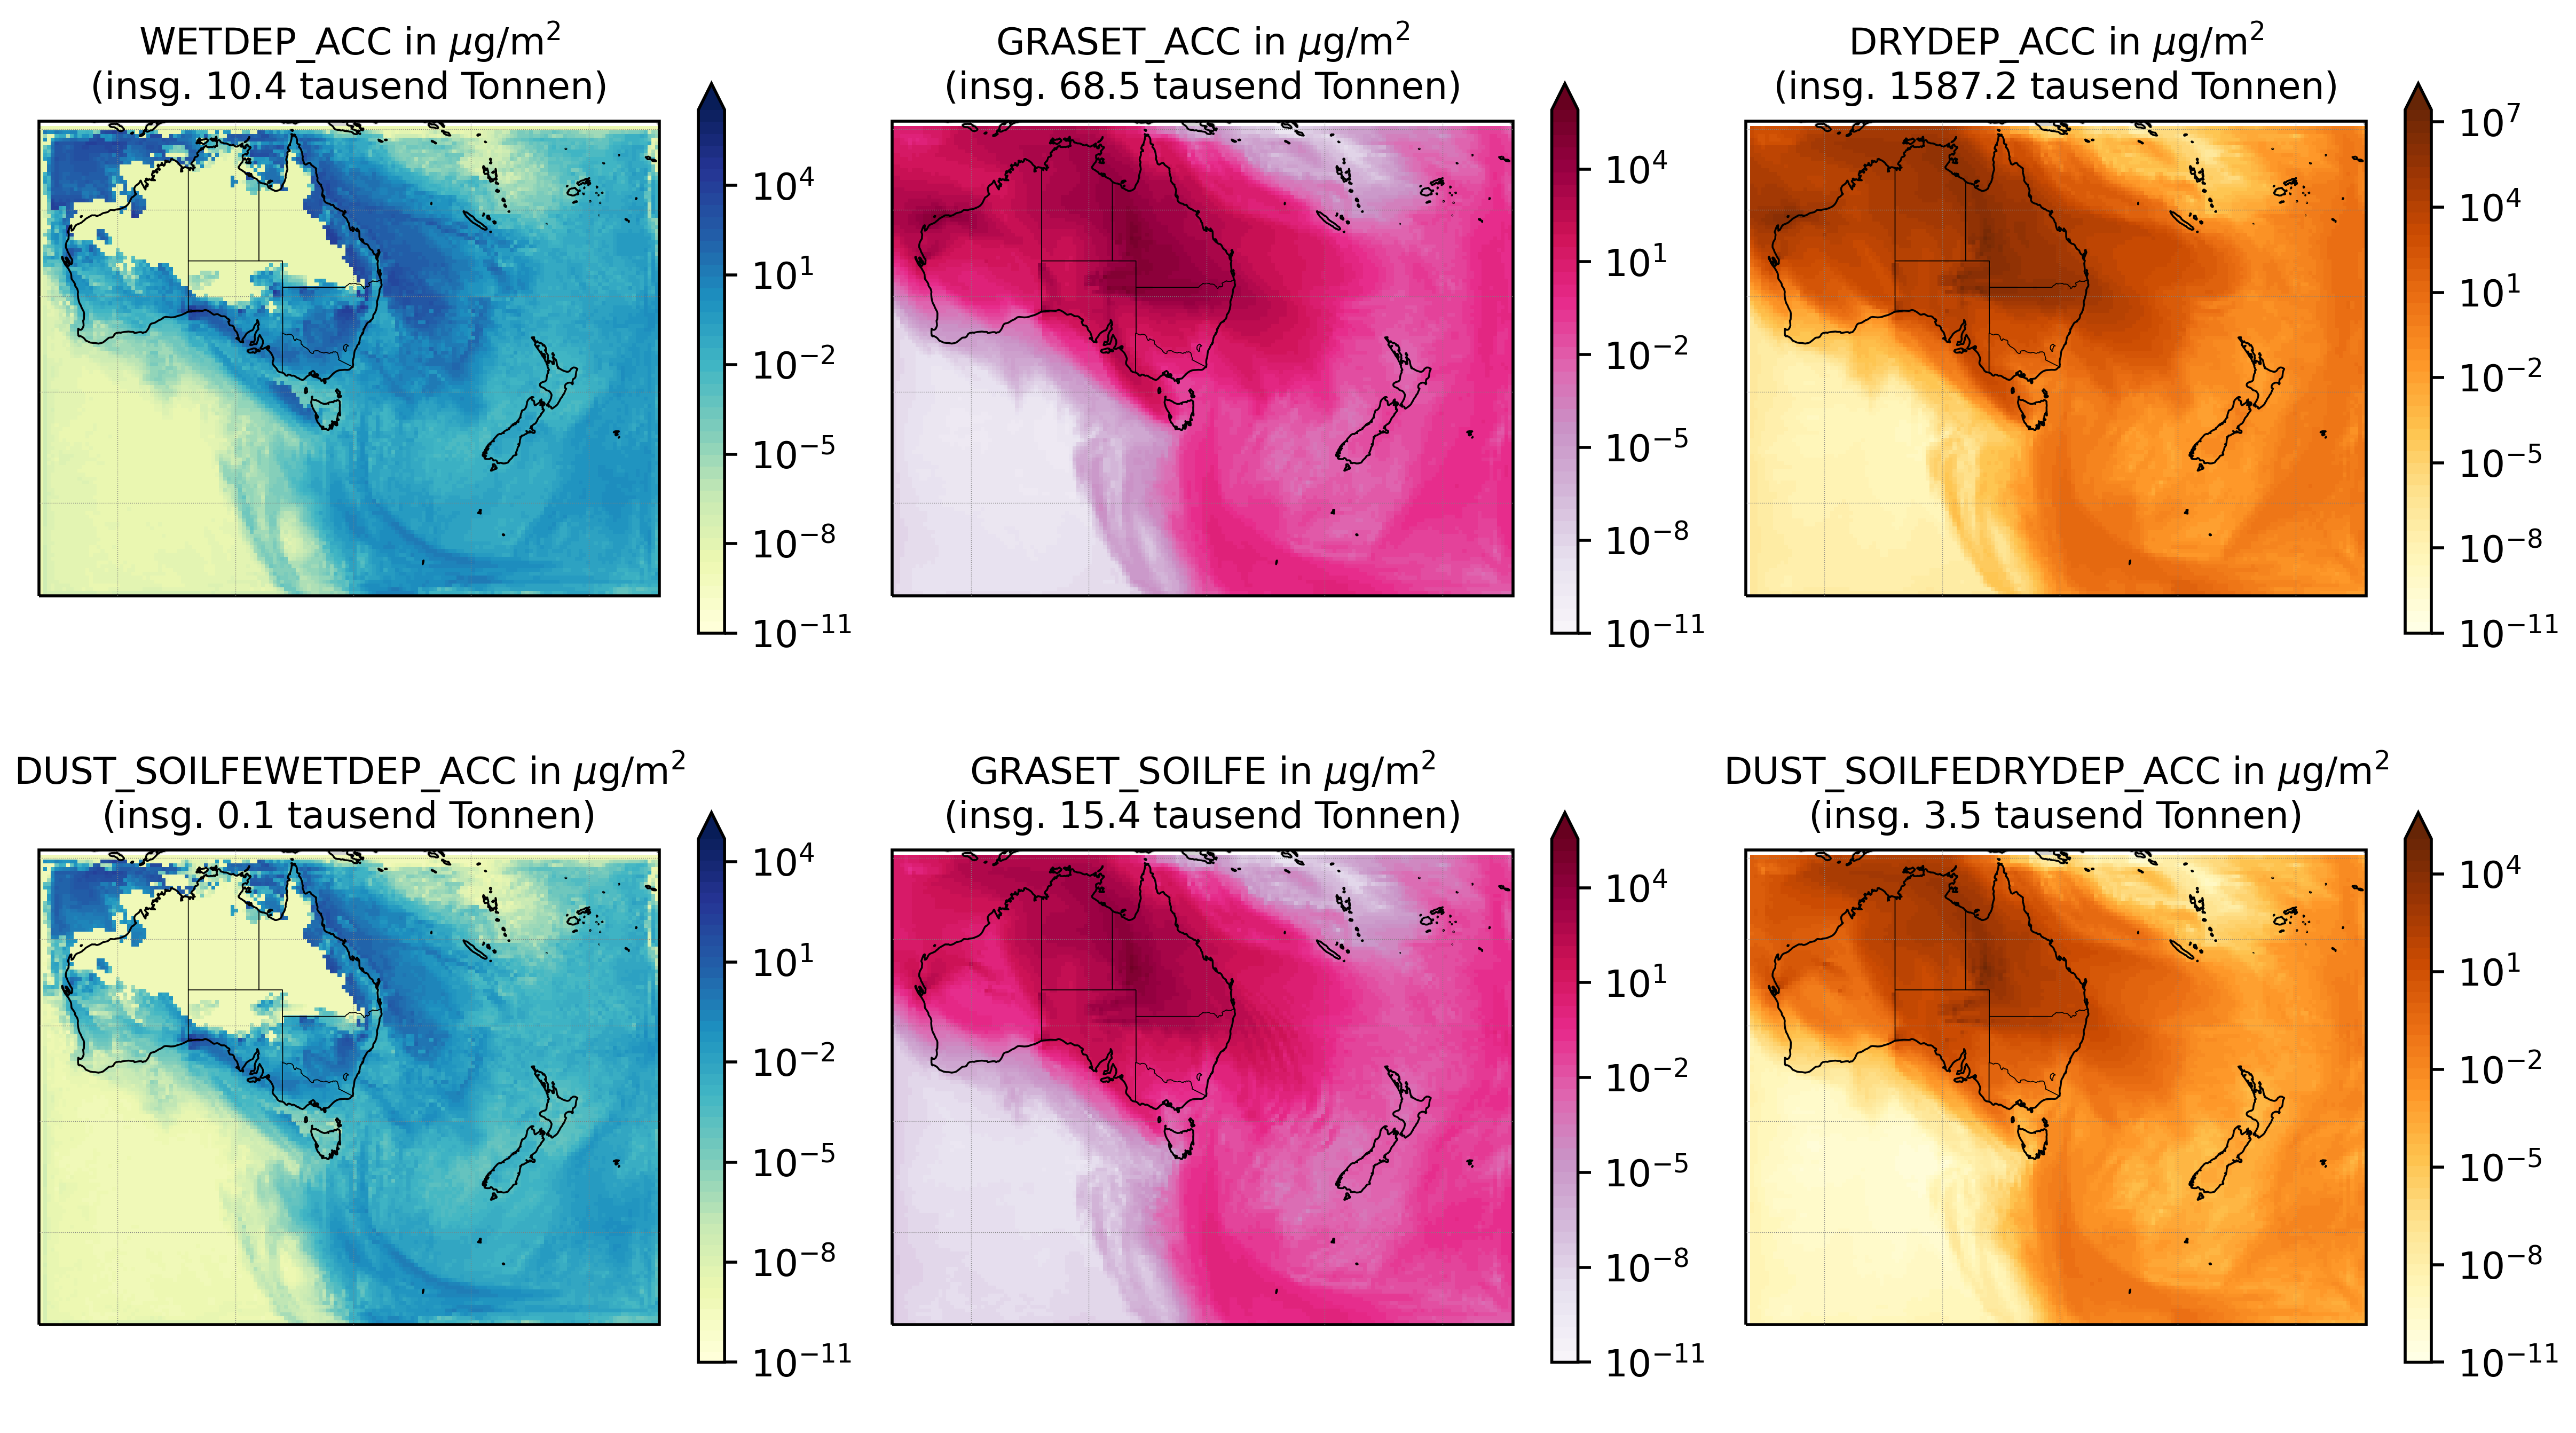
\includegraphics[width=\textwidth]{bilder/deposition.png}
\caption{Ergebnis des WRF-Modells: Der kumulierte Eintrag von Staub (oben) und Eisen (unten) über den gesamten Simulationszeitraum. Der Gesamteintrag ergibt sich als Summe von nassem Eintrag (links, Auswaschung durch Regen), Ablagerung durch Gravitation (Mitte) und trockenem Staubeintrag (rechts).} \label{fig:deposition}
\end{figure}
\subsection{Phytoplankton Reaktion}
\subsection{Anpassungen nach der ersten Simulation}
Die Ergebnisse der WRF-Simulation sollten in einem ersten Schritt durch eine grobe Übersicht auf Plausibilität, d.h. der wahrscheinlichen Abweichung von der Realität überprüft werden. Da ein relativ langer Zeitraum von 12 Tagen simuliert wird, sind auch größere Abweichungen wahrscheinlich. Ganz allgemein sind Wetterprognosen i.d.R. nur für die ersten Tage wirklich präzise. Die Wahrscheinlichkeit, dass das berechnete Wetter eintritt nimmt dann aufgrund des chaotischen Verhaltens der Atmosphäre und den beschränkt zur Verfügung stehenden diskreten Startwerten stark ab \textbf{(Quelle ergänzen)}. Beobachtungs- bzw. Reanalysedaten werden dem Modell zum Startzeitpunkt und an den Rändern geliefert. Die Zustände der zeitlich und räumlich dazwischen liegenden Gitterpunkte sind dann (ausschließlich) vom Modell simuliert (\textbf{Quelle Sven, nochmal checken}). Für den Großteil des untersuchten Gebietes liegen ohnehin keine Beobachtungsdaten vor. Der australische Kontinent ist relativ dünn mit Wetterstationen besetzt und Beobachtungen durch Satelliten sind hinsichtlich  zeitlicher und räumlicher Auflösung ebenfalls häufig relativ grob. Darüber hinaus können die interessanten Parameter meist nur indirekt ermittelt werden.
\\

Dennoch können einfache Vergleiche einen ersten Eindruck von der Qualität der Simulation vermitteln. Hierzu wurden die simulierten Staubkonzentrationen und Emissionen mit Satellitenbildern, Beobachtungsdaten und Schätzungen aus der diesbezüglichen Literatur verglichen. Der Abgleich mit den (Echt-Farben-) Satellitenbildern zeigt, dass die Fortbewegung und Ausdehnung der Staubwolke vom Modell grundsätzlich erfasst wird. Auf Abbildung \ref{fig:wrf_sat} ist jedoch ebenfalls gut sichtbar, dass das Modell zu späteren Zeiten eine deutlich höhere Staubkonzentration im Nordwesten Australiens simuliert, als von den Satellitenbildern direkt ableitbar wäre. Dabei ist zu beachten, dass die (Echt-Farben-) Satellitenbilder keine direkten Rückschlüsse auf die Staubkonzentration zulassen. Es können durchaus höhere Staubkonzentrationen vorliegen, die auf Satellitenbildern nicht erkannt werden können (\textbf{Behauptung Shao, Quelle ergänzen}). Aufgrund der dort simulierten sehr hohen Konzentrationen wird allerdings vermutet, dass entsprechende Emissionen überschätzt werden.

\begin{figure}[H]
	\begin{minipage}[c]{0.35\textwidth}
		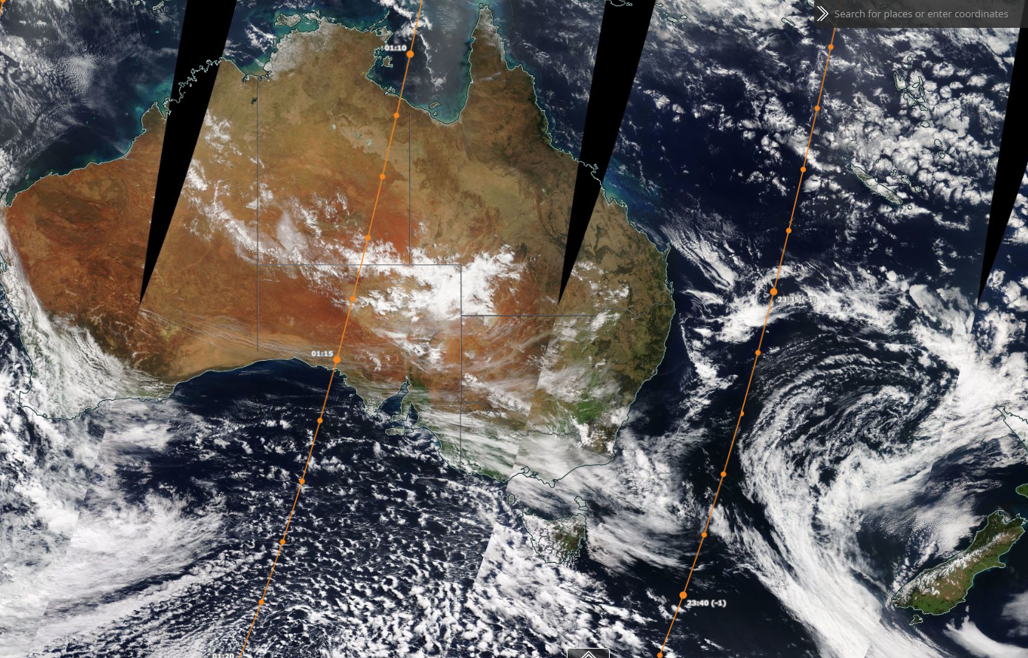
\includegraphics[width=\textwidth]{bilder/wrf/20T00_sat.png}
	\end{minipage}\hfill
	\begin{minipage}[c]{0.35\textwidth}
		 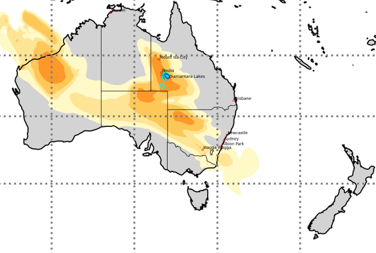
\includegraphics[width=\textwidth]{bilder/wrf/20T00_wrf.png}
	\end{minipage}\hfill
	\begin{minipage}[c]{0.29\textwidth}
		 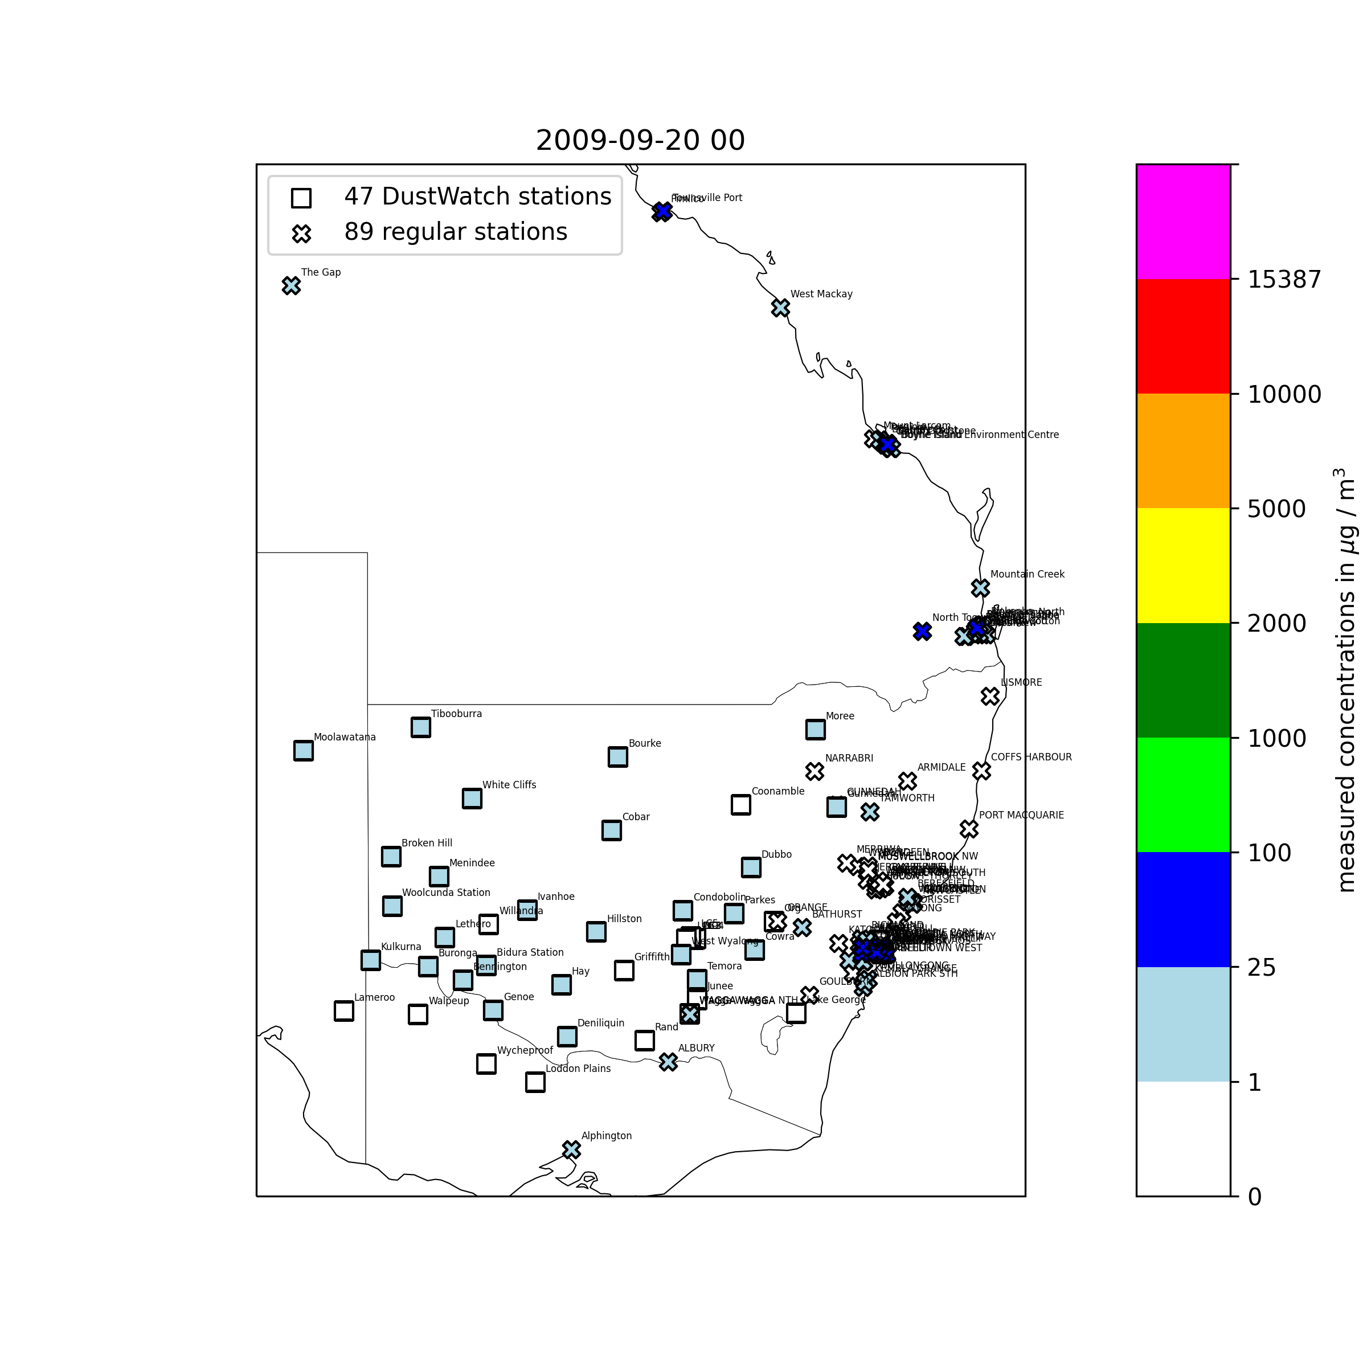
\includegraphics[width=\textwidth]{bilder/wrf/20T00_obs.png}
	\end{minipage}\hfill
	\begin{minipage}[c]{0.35\textwidth}
		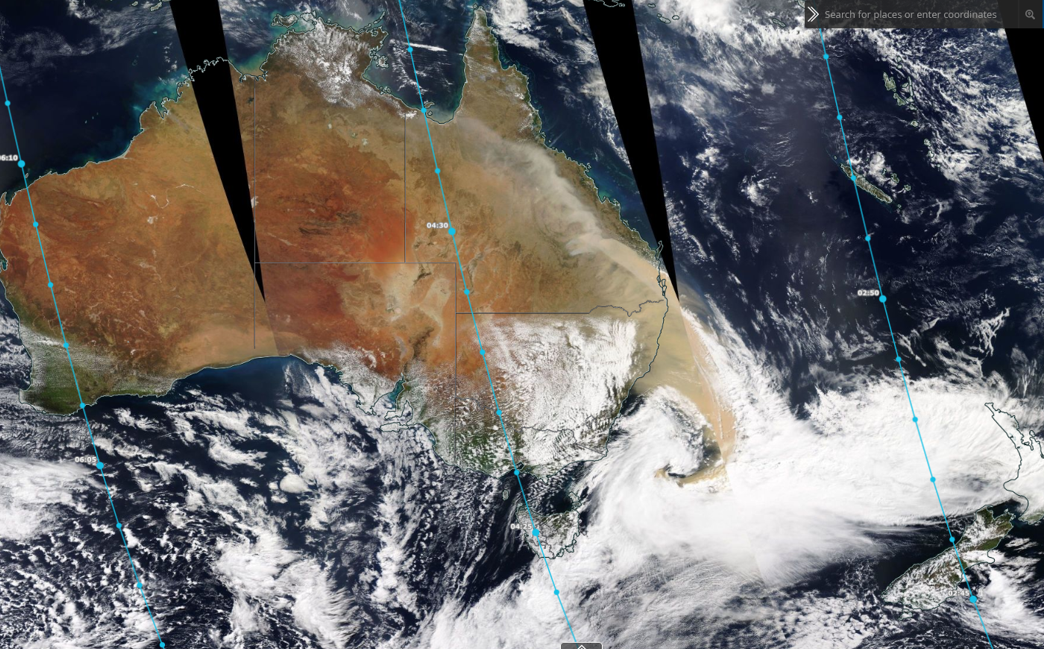
\includegraphics[width=\textwidth]{bilder/wrf/23T06_sat.png}
	\end{minipage}\hfill
	\begin{minipage}[c]{0.35\textwidth}
		 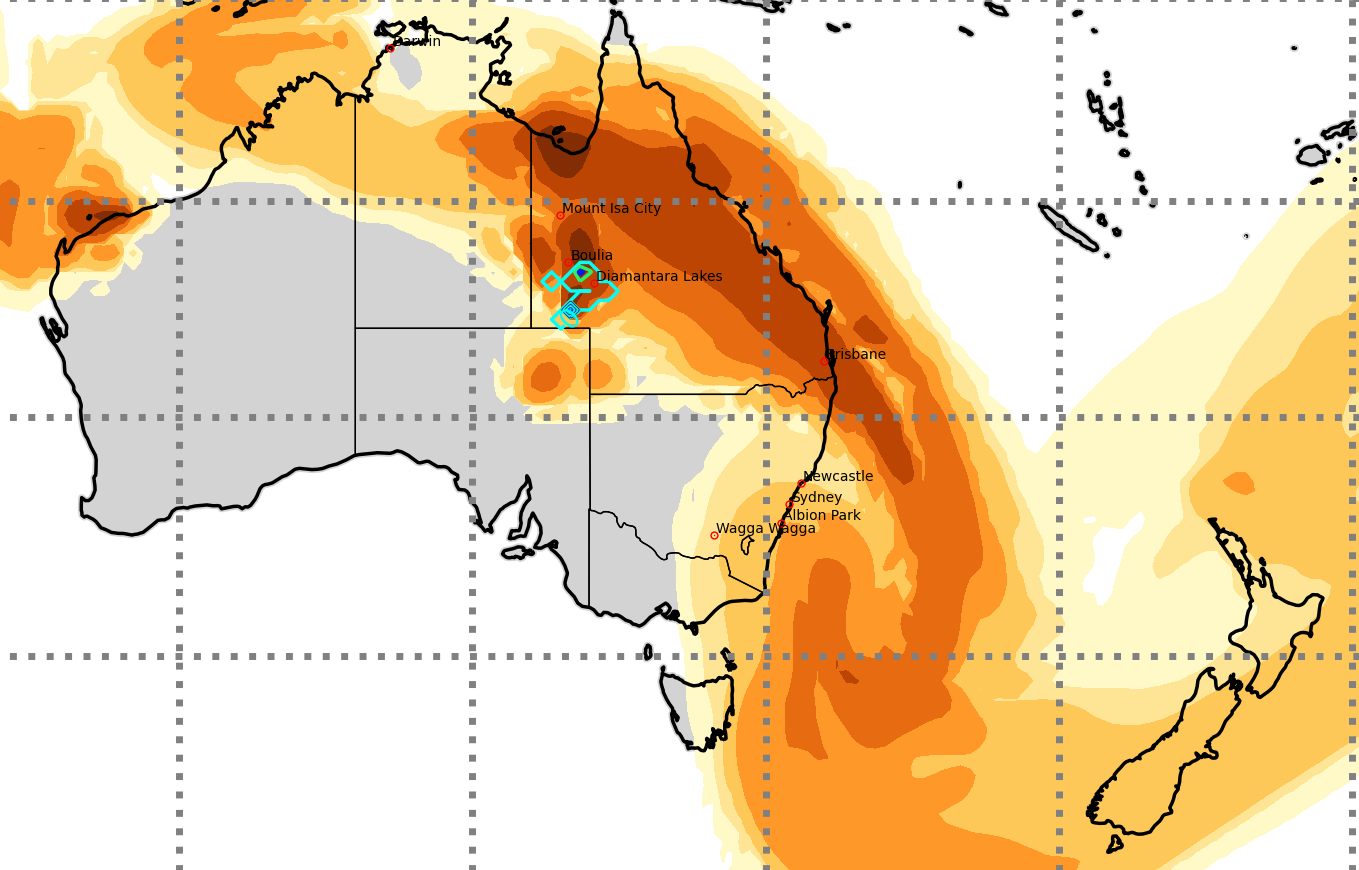
\includegraphics[width=\textwidth]{bilder/wrf/23T06_wrf.png}
	\end{minipage}\hfill
	\begin{minipage}[c]{0.29\textwidth}
		 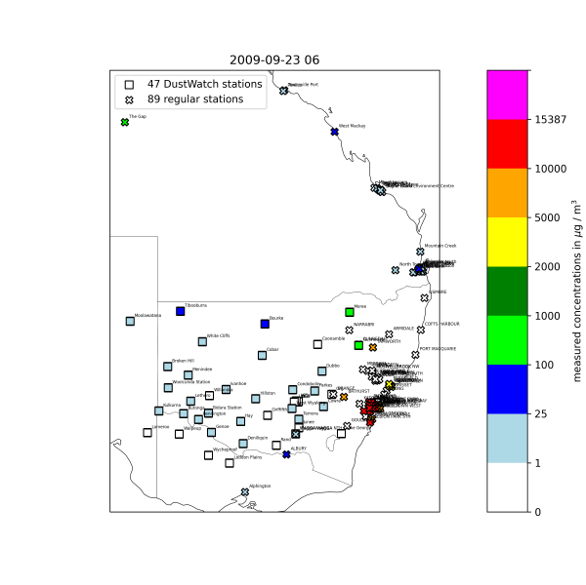
\includegraphics[width=\textwidth]{bilder/wrf/23T06_obs.png}
	\end{minipage}\hfill
	\begin{minipage}[c]{0.35\textwidth}
		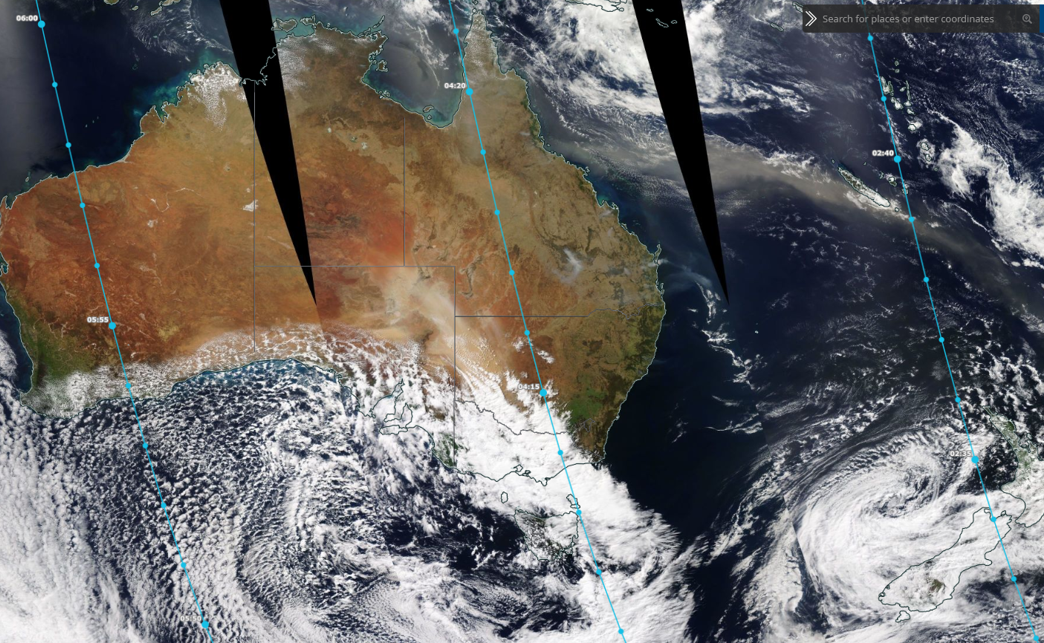
\includegraphics[width=\textwidth]{bilder/wrf/25T06_sat.png}
	\end{minipage}\hfill
	\begin{minipage}[c]{0.35\textwidth}
		 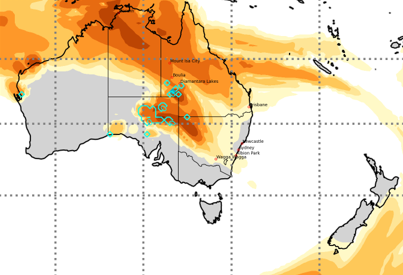
\includegraphics[width=\textwidth]{bilder/wrf/25T06_wrf.png}
	\end{minipage}\hfill
	\begin{minipage}[c]{0.29\textwidth}
		 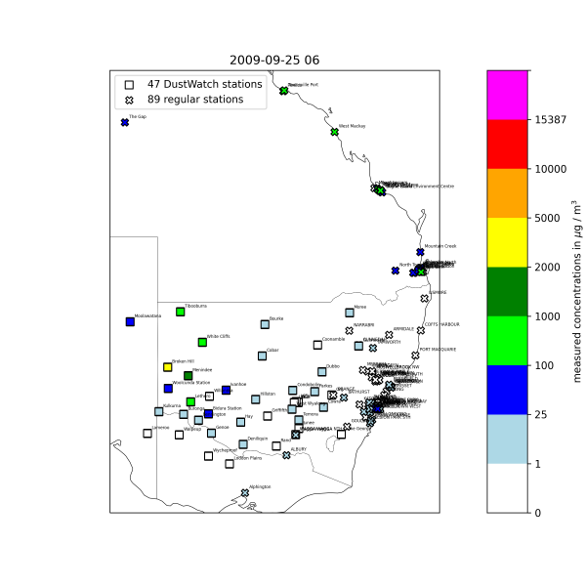
\includegraphics[width=\textwidth]{bilder/wrf/25T06_obs.png}
	\end{minipage}\hfill
	\begin{minipage}[c]{\textwidth}
		\captionsetup{format=hang, indention=0.0cm}
		\caption{Das muss ich irgendwie noch schöner machen....}
		\label{fig:wrf_sat}
	\end{minipage}
\end{figure}
Der Großteil des Staubs wird laut WRF-Modell aus der Region \textit{Channel Country} im Westen Queensland in der Nähe der \textit{Diamantina Lakes} emittiert. Diese Region wird grundsätzlich als Quelle für das Red-Dawn-Event vermutet (sh. Kapitel \textbf{XY}, \cite{Leys.2011}), allerdings bislang nicht als dominierende. Auf Abbildung \ref{fig:max_emis} wird deutlich, dass diese im Modell aber deutlich dominiert. Die Vermutung liegt nahe, dass ebendiese Emissionen zu den erhöhten (möglicherweise unrealistischen) modellierten Staubkonzentrationen im Nordwesten führen. Die Staubemissionen können im Modell aus verschiedenen Gründen überschätzt werden. Ein offensichtlicher Nachteil des im Modell implementierten Schemas zur Staubemission ist, dass nicht berücksichtigt wird, wie viel Staub am jeweiligen Gitterpunkt maximal emittiert werden kann. Ist eine Region also einmal als Staubquelle mit einer entsprechenden Größenordnung definiert, kann bei entsprechenden Windstärken theoretisch beliebig viel Staub emittiert werden. Dies soll in späteren Versionen durch eine \textit{Budgetierung} des maximal \textit{emissionsfähigen} Staubs an der Oberfläche implementiert werden, sodass die Emission stoppt, nachdem das Budget aufgebraucht ist. Durch neue Ablagerungen von Staub (Deposition) kann das Budget dann wieder aufgefüllt werden. Anschließend wären die Emissionen \textit{zeitlich} limitiert.
\begin{figure}[H]
\centering
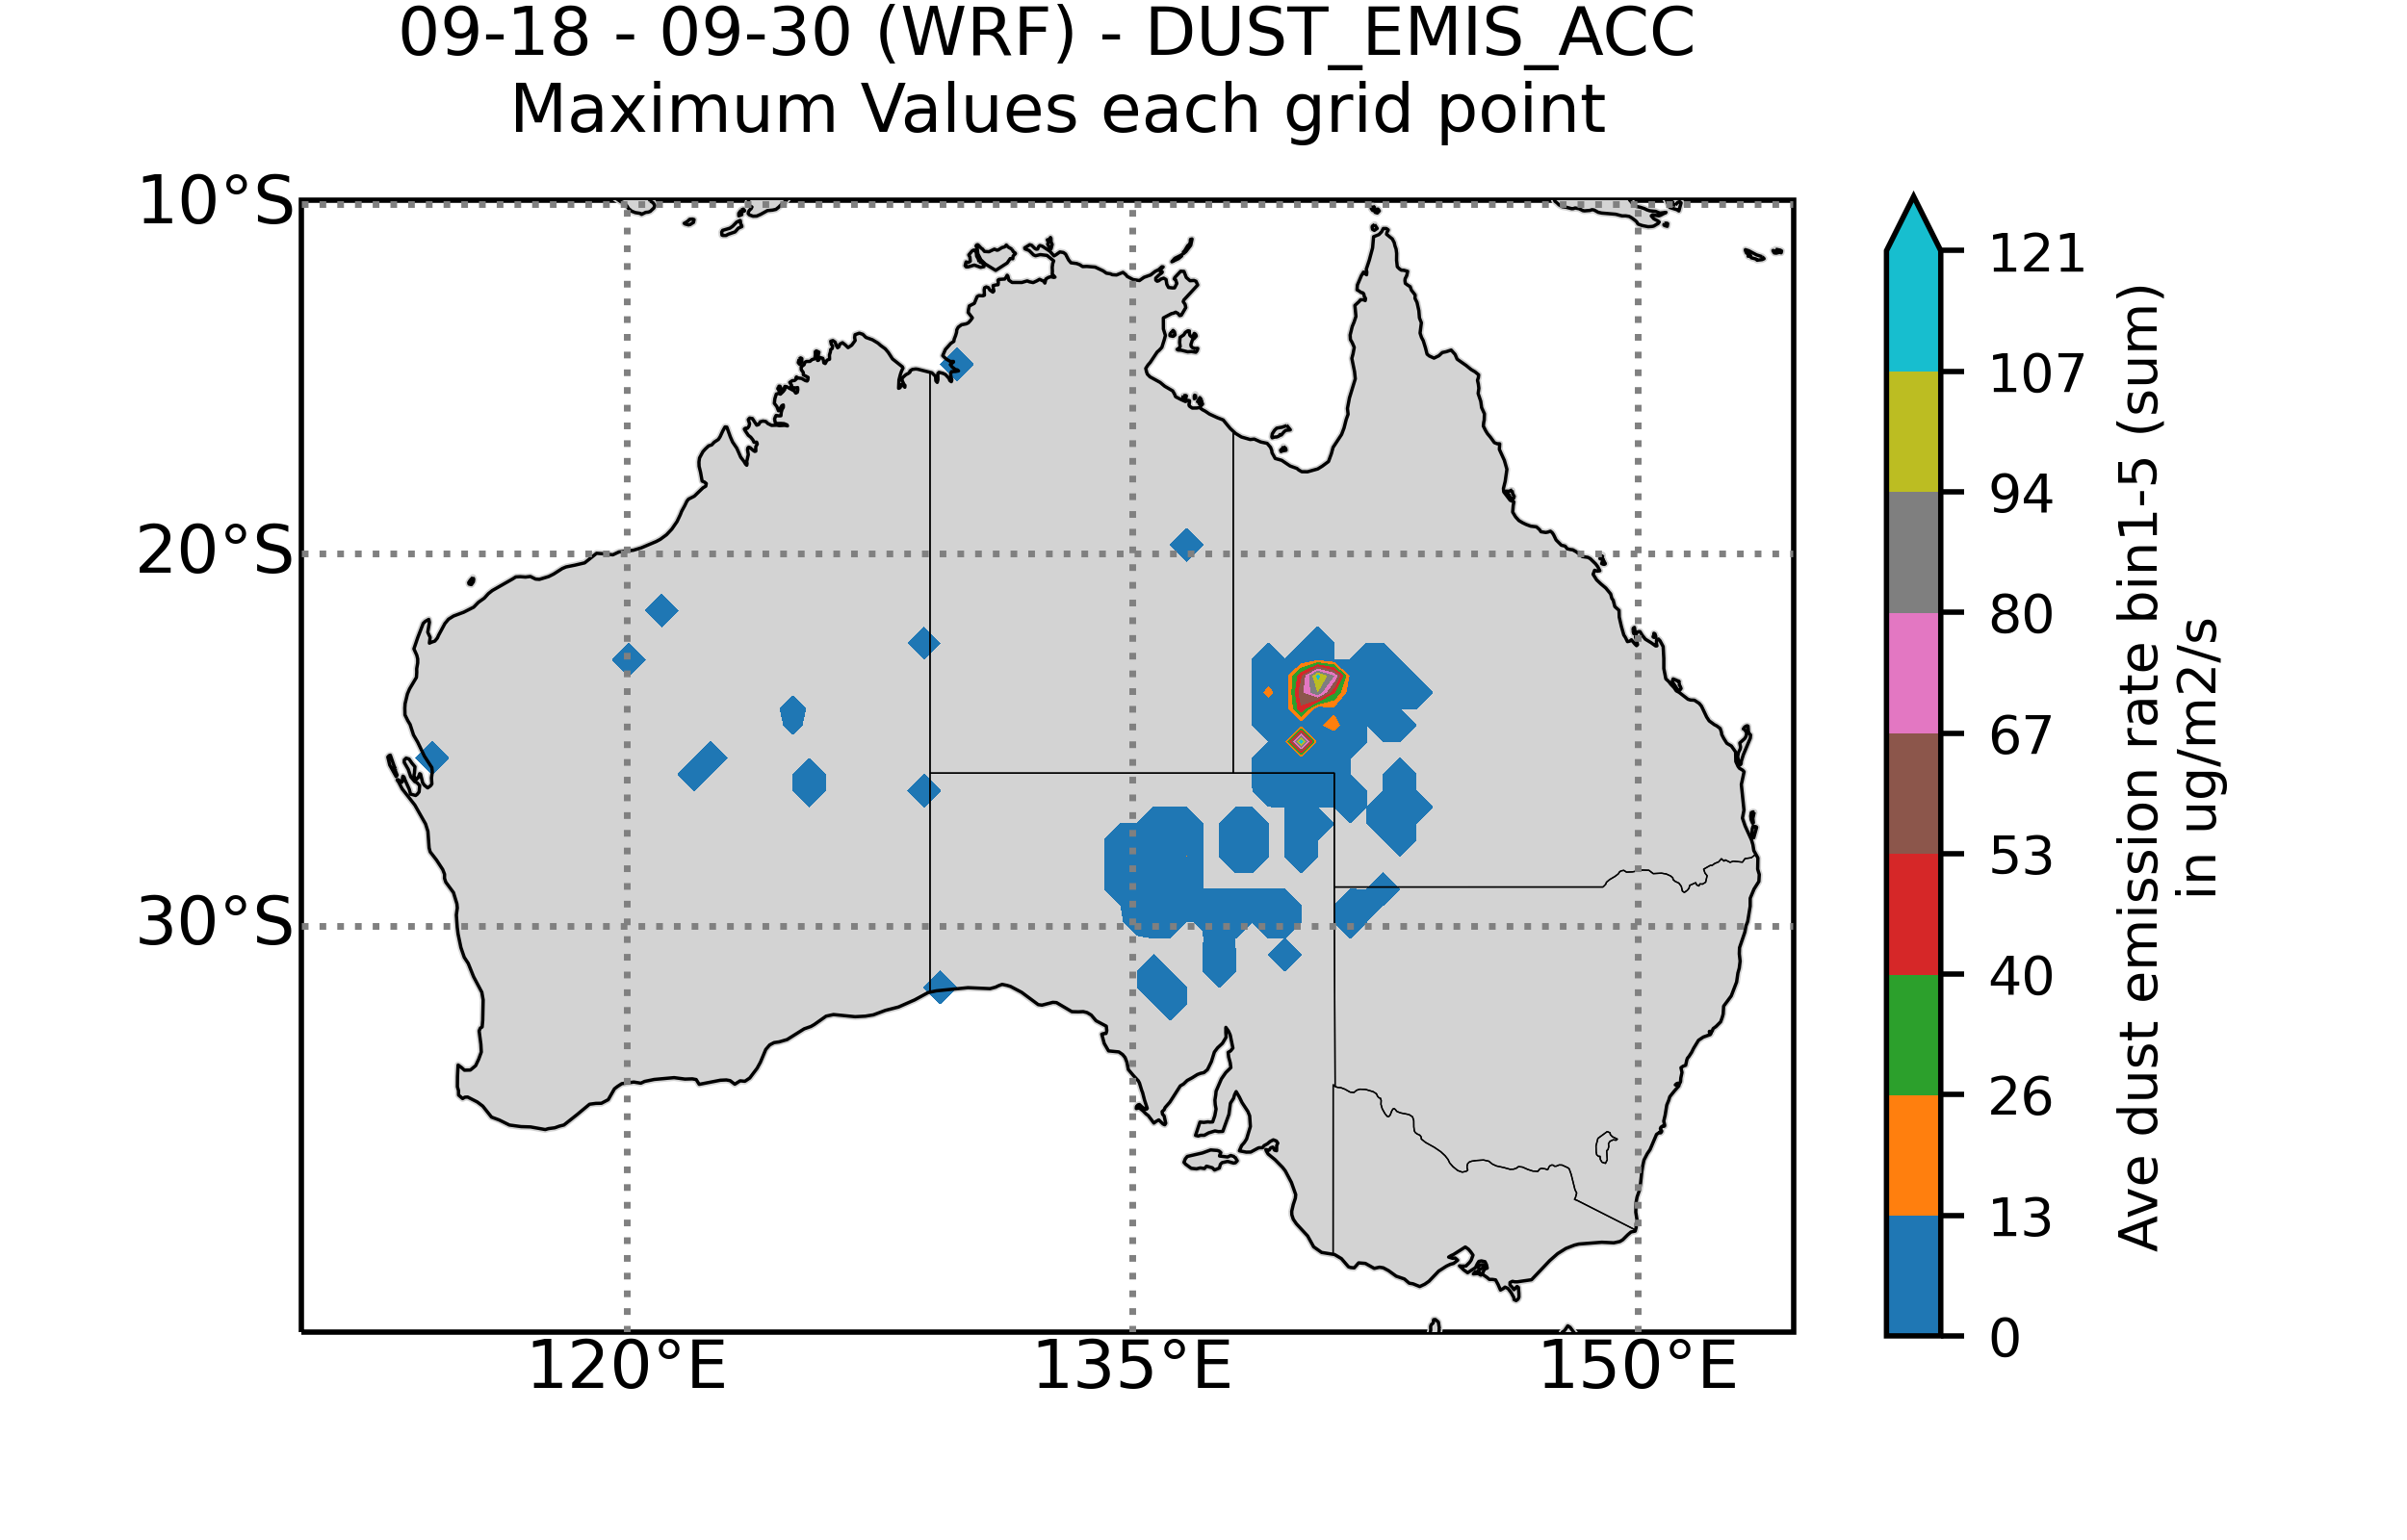
\includegraphics[width=\textwidth]{bilder/wrf/max_emis.png}
\caption{Darstellung der maximalen Staubemissionen über alle Zeiten je Gitterpunkt. Die Variablen DUST_EMIS_ACC1..5 beschreiben die über den letzten Zeitschritt (hier 3 Stunden) gemittelten Werte der Staubemissionen und wurden hier aufsummiert.} \label{fig:max_emis}
\end{figure}
Neben der zeitlichen Beschränkung beeinflussen verschiedene Parameter die zeitunabhängige Größenordnung der Emissionen. Insbesondere entscheidend für das Emissionspotential ist die Rauheit des Geländes. Dies stellt in Simulationen stets ein Problem dar, da die räumliche Auflösung eines diskreten Modells nie alle beliebig kleinen Elemente abdecken kann. Stattdessen wird jedem Gitterpunkt ein Parameter zugeordnet, der die Rauheit repräsentiert und die Emissionen stellvertretend regulieren soll. Im vorliegenden WRF-Modell werden dazu die Vegetationsparameter angepasst \textbf{LAI oder VEGFRA?}, da Vegetation einen vergleichbaren Einfluss nimmt wie Rauheit, bzw. ebenfalls eine gewisse Rauheit darstellt. Diese Informationen, welche Größe die Parameter an welchem Gitterpunkt annehmen, werden durch Geogrid-Daten in das WRF-Modell gegeben. In Abbildung \label{fig:emis_ctrl} sind einige der relevanten Parameter dargestellt. Es wird deutlich, dass die Zelle mit den höchsten Emissionen (\textit{1}) im Vergleich zu den Nachbarzellen etwas andere Werte erreicht, was zu verstärkten Emissionen führt. Da angenommen wird, dass die sehr hohen Emissionen unrealistisch sind, wurde der Blattflächenindex (LAI) an den 10 Gitterpunkten mit den höchsten Emissionen gezielt korrigiert. Dies führt zu einer veränderten Rauheit und soll die Emissionen auf ein adäquates Level limitieren.

\begin{figure}[H]
\centering
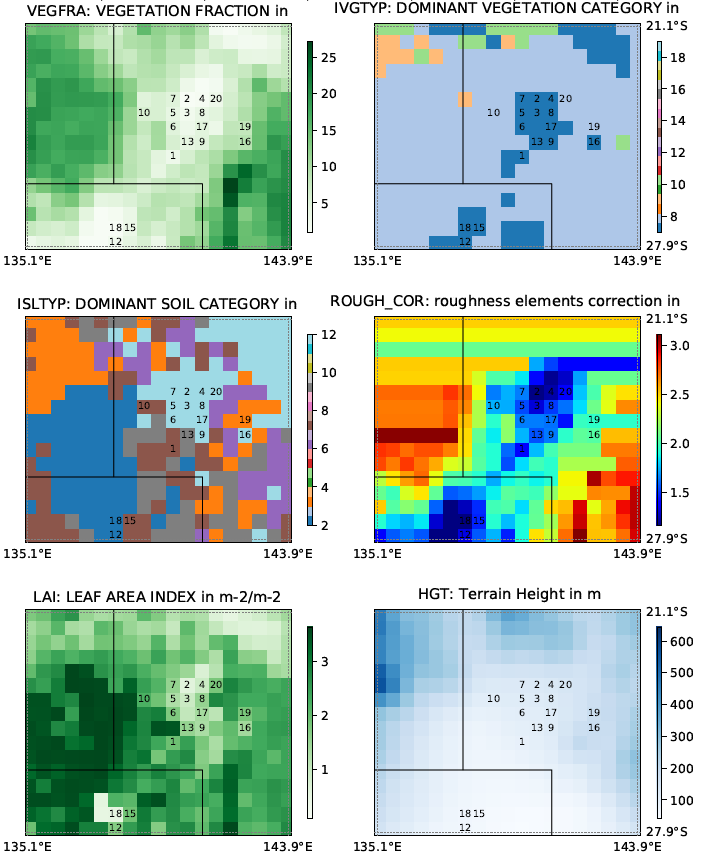
\includegraphics[width=0.7\textwidth]{bilder/wrf/emis_ctrl.png}
\caption{Absolute Werte einiger konstanter Parameter im WRF-Modell für die Region mit hohen Emissionen, die die Staubemissionen regulieren können. Die Zahlenwerte 1 bis 20 geben die Rangordnung der Staubemissionen an. Das heißt, Gitterpunkt 1 erreicht die höchste Emission, 2 die zweithöchste usw.}

\end{figure}



\subsection{Staubkonzentrationen}
- Hohe Konzentrationen an der Oberfläche werden durch Modell ungenügend beschrieben (siehe DUST_ACC_ auf zlevel 0 (geländefolgend)). DUSTLOAD über ganze Atmosphärensäule allerdings schon eher. Sehr sehr hohe Konzentrationen  ($>$ 10kg pro qm) später im Norden.
\section{Staubquellen und Emissionen}
Staubquellen gemäß \citep{Leys.2011}
\begin{enumerate}
\item lower Lake Eyre Basin
\item grazing lands of north western NSW
\item mining areas around Cobar und Broken Hill
\item Channel Country of western Queensland
\end{enumerate}
Laut Modell enorm hohe Emissionen zwischen Diamantara Lakes und Boulia (western Queensland). Laut \citet{Deckker.2014} konnte Lake Torrins als Quelle für Staub der bei Canberra gefallen ist identifiziert werden. Diese Region ebenfalls Bestandteil des Modells. Die \textit{Fingerabdruckanalyse} von \citet{Deckker.2014} ist leider dadurch beschränkt, dass nur Proben aus den beiden (im Vergleich zur Ausdehnung der Staubwolke) sehr südlich gelegenen Städten Canberra und Eden verwendet werden konnten. Die damit abgeleiteten Staubquellen sind also vermutlich für den Großteil des Ereignisses nicht repräsentativ. -  Benutzt man die Unterteilung in \citet{OLoingsigh.2017}, dann laut Modell Region (2) Channel Country mit Abstand größte Quelle, aber auch (3) Lake Eyre (A) and South Simpson desert ephemeral lakes region, (4) South Strzelecki desert and Lake Frome (B) subbasin, (5) Lakes Torrens (C). -  Staub beschreibt eine bestimmte Signatur, die von den Eigenschaften des Sediments unterschieden werden kann, in welchem sich der Staub abgelagert hat. Die besondere Signatur kann nach \citet{Marx.2018} durch verschiedene Mechanismen verursacht werden:
\begin{enumerate}
\item Transport
\item geochemisch oder mineralogisch
\item \textit{Fingerabdruck} der Herkunftsregion
\item anthropogene Effekte
\end{enumerate}
\section{Zusammenfassung und Ausblick}
\newpage
\printbibliography
\appendix
\section{Anhang}
\addcontentsline{toc}{section}{Abbildungsverzeichnis}
\listoffigures
\addcontentsline{toc}{section}{Tabellenverzeichnis}
\listoftables
\section{Danksagung}
\nocite{*}
\end{document}
